\chapter{Evaluation}
\label{sec:evaluation}

% Zu jeder Arbeit in unserem Bereich gehört eine Leistungsbewertung. Aus
% diesem Kapitel sollte hervorgehen, welche Methoden angewandt worden,
% die Leistungsfähigkeit zu bewerten und welche Ergabnisse dabei erzielt
% wurden. Wichtig ist es, dem Leser nicht nur ein paar Zahlen
% hinzustellen, sondern auch eine Diskussion der Ergebnisse
% vorzunehmen. Es wird empfohlen zunächst die eigenen Erwartungen
% bezüglich der Ergebnisse zu erläutern und anschließend eventuell
% festgestellte Abweichungen zu erklären.
The previous chapters have analyzed the security issues associated with the OCI runtime interface in confidential computing, and have proposed the design and implementation of a shielding layer as a countermeasure. Therefore, this chapter assesses the security and performance of the implementation 
from both qualitative and quantitative viewpoints. A brief introduction to qualitative and quantitative analyses can be found in Section~\ref{sec:eva_qualitativ} and~\ref{sec:eva_overwiwe_Quantitative}.
Note that the implementation is referred to as confidential Quark in the subsequent discussions.


\section{Qualitative Analysis}
\label{sec:eva_qualitativ}
The qualitative analysis employs a microbenchmark to evaluate the effectiveness of the system implemented in Chapter~\ref{sec:implementation} in mitigating vulnerabilities of the OCI runtime interface listed in Section~\ref{sec:security_analyse_oci_summary}. The setup of the 
microbenchmark is described in Subsection~\ref{sec:eva_qualitativ_setup}. Next, Subsection~\ref{sec:eva_qualitativ_secure_depl} demonstrates the secure deployment process for an application. Subsection~\ref{sec:eva_qualitativ_secure_exec} further assesses how the shield performs authentication and access control on EXEC requests.
Subsection~\ref{sec:eva_qualitativ_secure_stdio} then illustrates the shield can cryptographically protect the process STDIO. Finally, Subsections~\ref{sec:eva_qualitativ_secure_log},~\ref{sec:eva_qualitativ_secure_syscall}, and~\ref{sec:eva_qualitativ_runtime_meausre}
highlight the shield's ability to manage VM logs, restrict available system calls to the application, and ensure the integrity of executables loaded from the host while \acrshort{CVM} runs, respectively. A summary of the qualitative analysis can be found in Subsection~\ref{sec:eva_qualitativ_summary}.


\subsection{Common Setup}
\label{sec:eva_qualitativ_setup}

This section outlines the configuration for the analysis. First, the environment of confidential and vanilla Quark is set following the guidelines provided in the Quark demo repository~\cite*{Qaurk_Demo_for_qualitativ}. The policy used by the confidential Quark is shown in Figure~\ref{fig:generic_policy}. 
The policy specifies that the shield is in \texttt{Production} mode. Privileged users can allocate terminals and issue \texttt{cat} and \texttt{ls} commands, while non-privileged level users can only issue \texttt{ls} commands. Privileged-level commands can be executed in the directory 
\texttt{/var} and its subdirectories, while non-privileged-level commands can only access the directory \texttt{/var/log} and its subdirectories. In addition, the Qlog manager is turned on. Since \emph{allowed\_max\_log\_level} is set to \texttt{OFF}, the Qkernel of the confidential Qaurk does 
not print any logs. Finally, the guest system call interceptor is activated and runs in \texttt{ContextBase} mode. The system call allowlist contains all system calls (0-451), some of which are not included in the figure due to space limitations.


\begin{figure}[!htb]
  \centering
  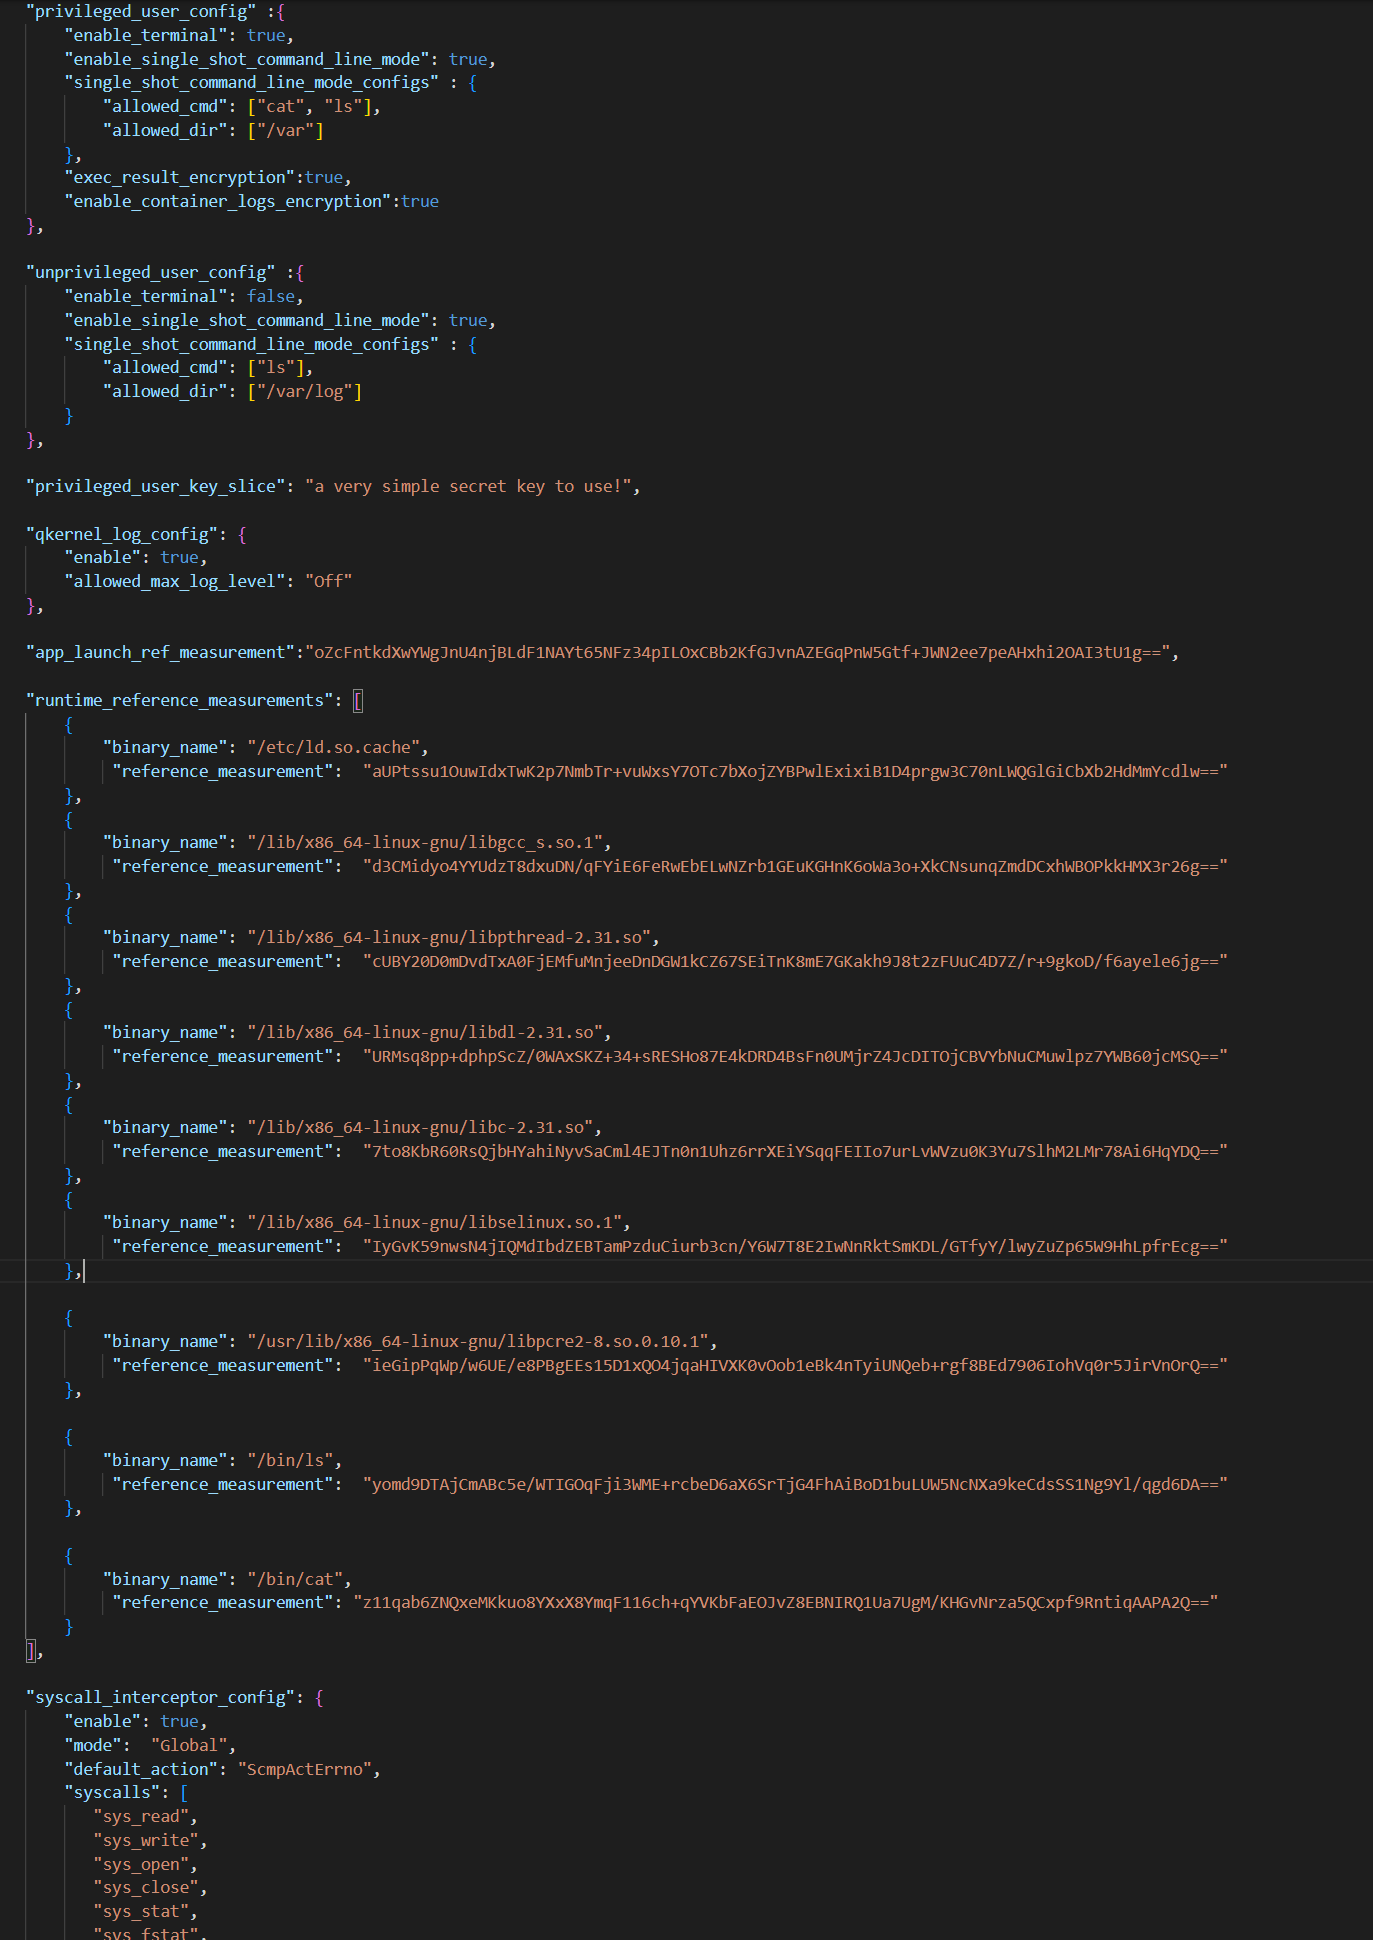
\includegraphics[height=0.3\textheight]{images/generic_policy.PNG}
  \caption[Shield policy for confidential Quark]{Shield policy for confidential Quark}
  \label{fig:generic_policy}
\end{figure}


% \begin{figure}[!htb] 
%   \begin{subfigure}[b]{0.45\linewidth}
%     \centering
%     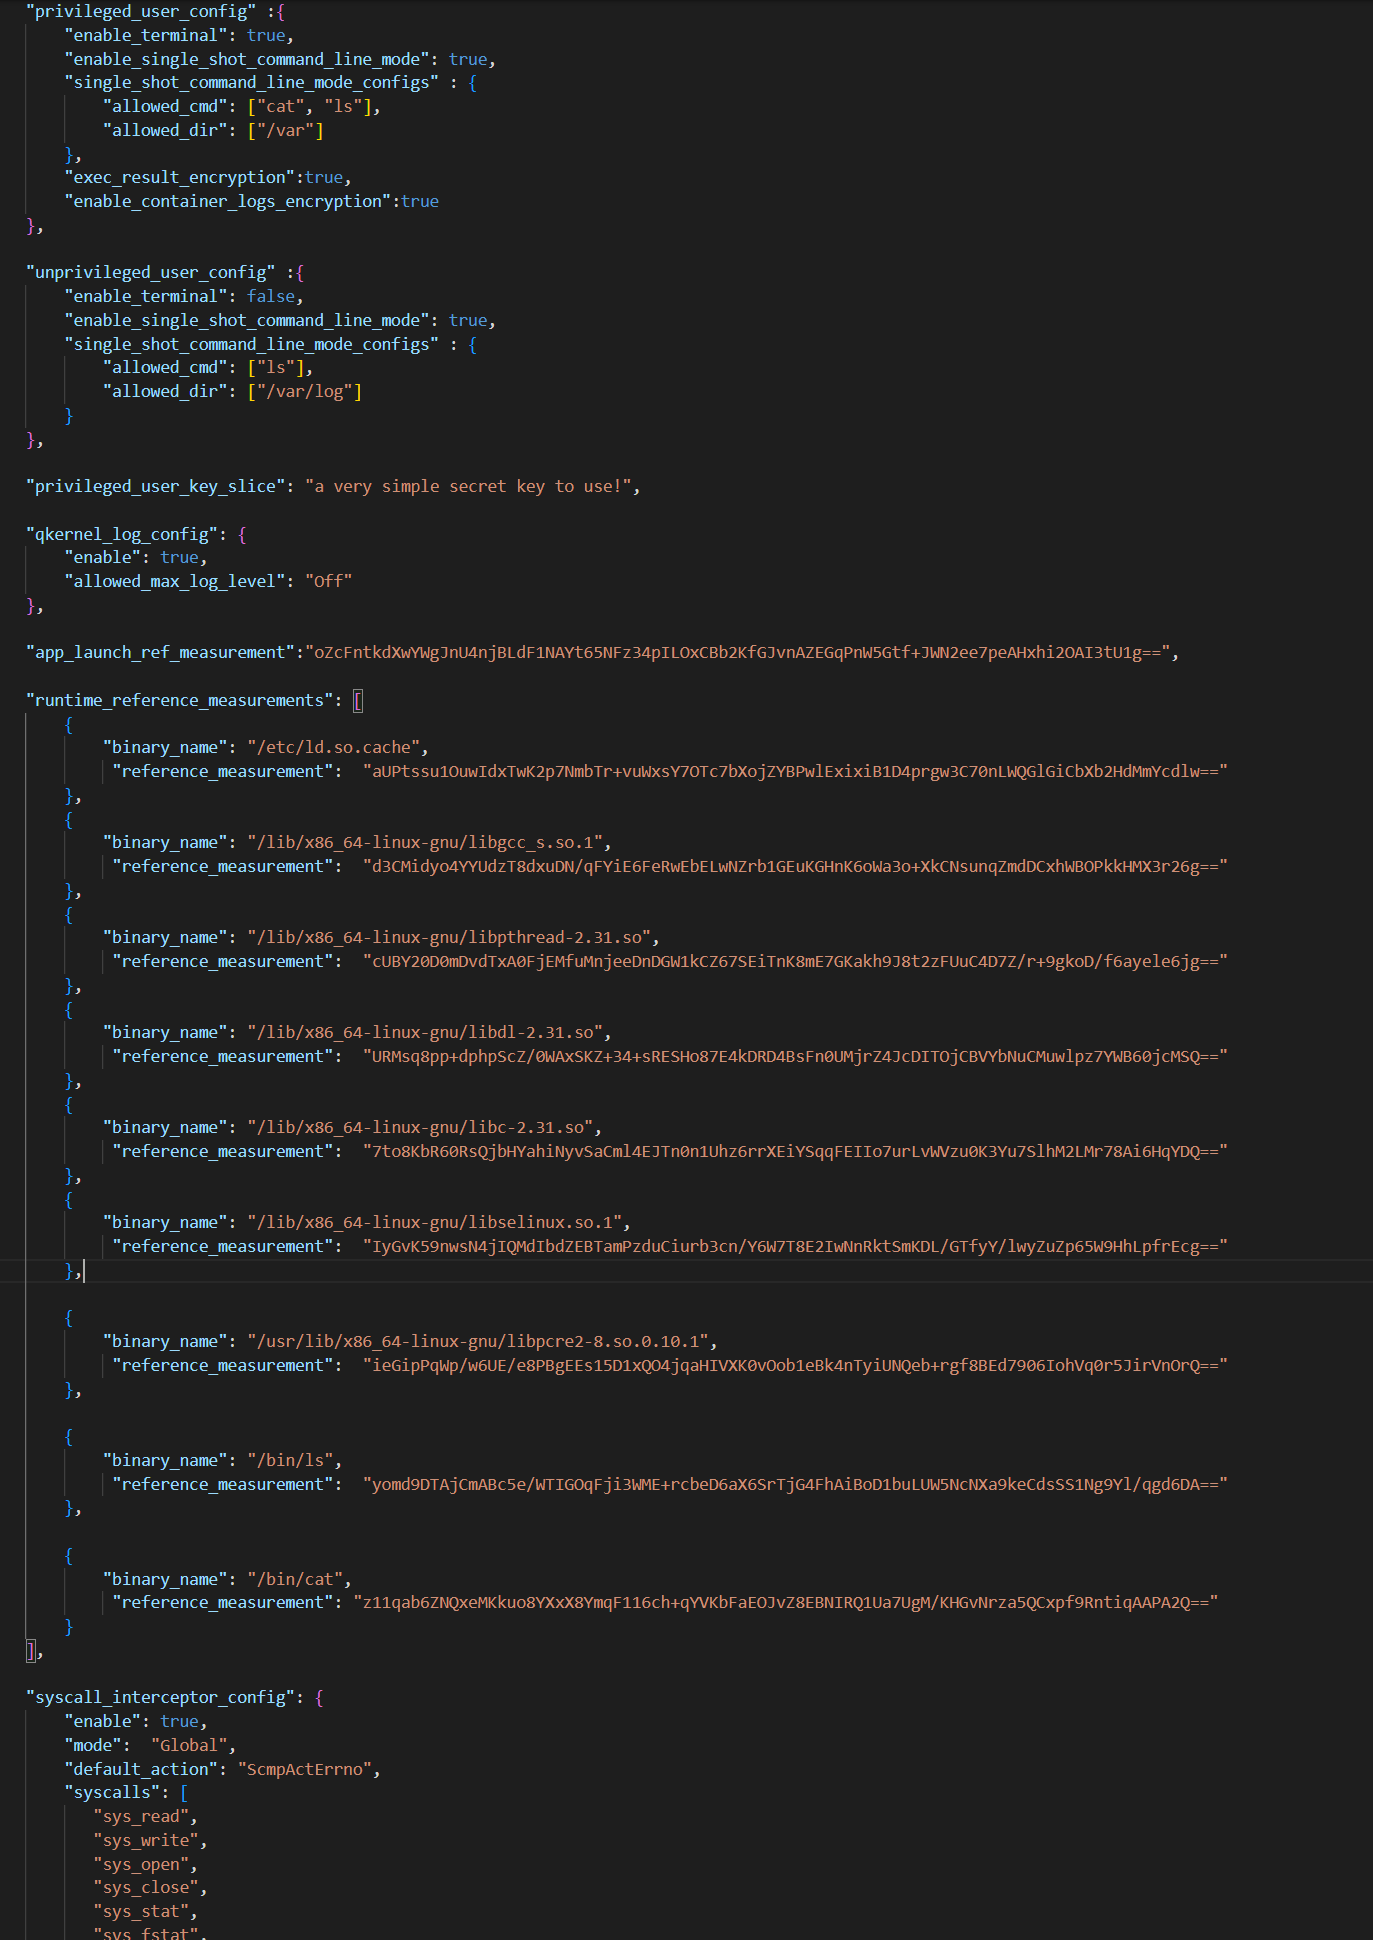
\includegraphics[width=0.9\linewidth]{images/generic_policy.PNG} 
%     \caption{Enclave policy} 
%     \label{fig:generic_policy} 
%     \vspace{4ex}
%   \end{subfigure}%% 
%   \begin{subfigure}[b]{0.45\linewidth}
%     \centering
%     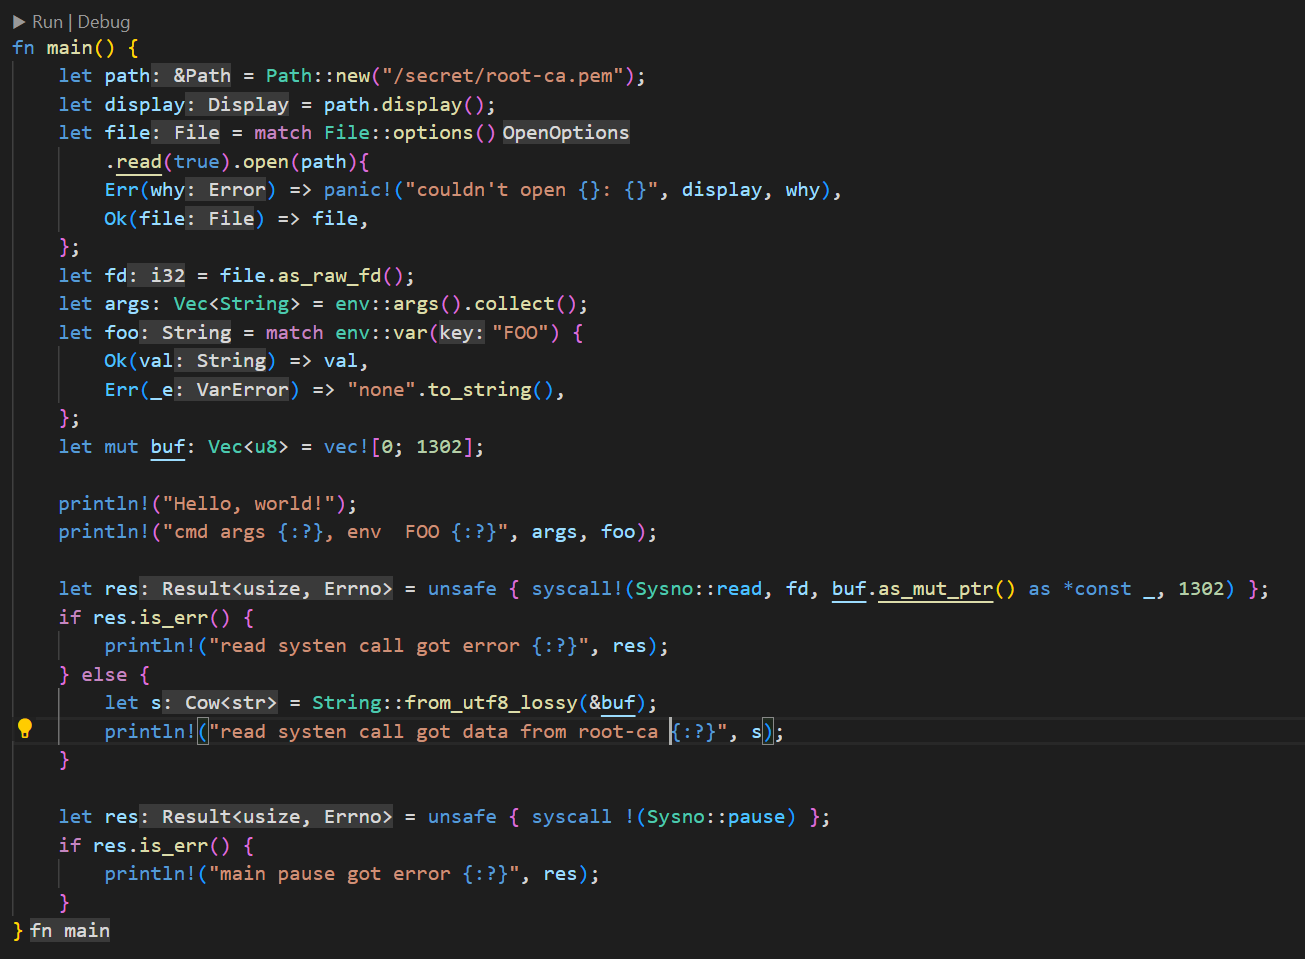
\includegraphics[width=0.9\linewidth]{images/analysis_workload.png} 
%     \caption{Program used for the qualitative analysis} 
%     \label{fig:analysis_workload} 
%     \vspace{4ex}
%   \end{subfigure} 
%   \caption{Artifacts for demo in the qualitative analysis}
%   \label{fig4} 
% \end{figure}

The analysis uses a simple program~\cite*{qualitativ_programs} to demonstrate the functionality of confidential Quark. The program first prints the application's environment variable and startup parameter type secrets. Then it reads the first few lines of the file type 
secret \textbf{/secret/root-ca.pem} and prints the result. The application-related secrets are shown in Figure~\ref{fig5}. The script~\cite*{secret_uploading_script} is utilized to deploy these secrets and the shield policy to the secret manager. Note that the program is already 
containerized. The artifacts for the demo in the qualitative analysis and the YAML files for deploying the demo can be found in commit~\cite*{artifacts_quarlitative}.

\begin{figure}[!htb] 
    \begin{subfigure}[b]{0.45\linewidth}
      \centering
      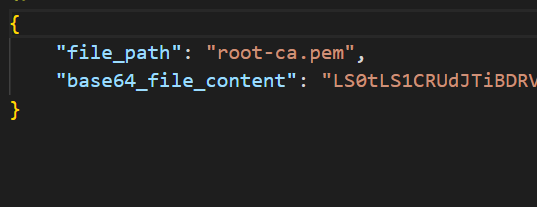
\includegraphics[width=0.9\linewidth]{images/file_secrets.PNG} 
      \caption{File type secrets} 
      \label{fig:file_secrets} 
      \vspace{4ex}
    \end{subfigure}%% 
    \begin{subfigure}[b]{0.45\linewidth}
      \centering
      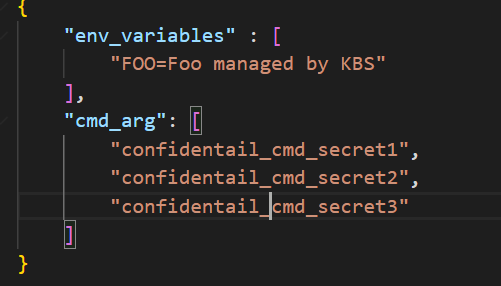
\includegraphics[width=0.9\linewidth]{images/cmd_env_secrets.png} 
      \caption{Args and Envv based secrets} 
      \label{fig:cmd_env_secrets} 
      \vspace{4ex}
    \end{subfigure} 
    \caption{Secrets for demo in the quantitative analysis}
    \label{fig5} 
\end{figure}


\subsection{Secure Application Deployment}
\label{sec:eva_qualitativ_secure_depl}
\begin{figure}[!htb]
    \centering
    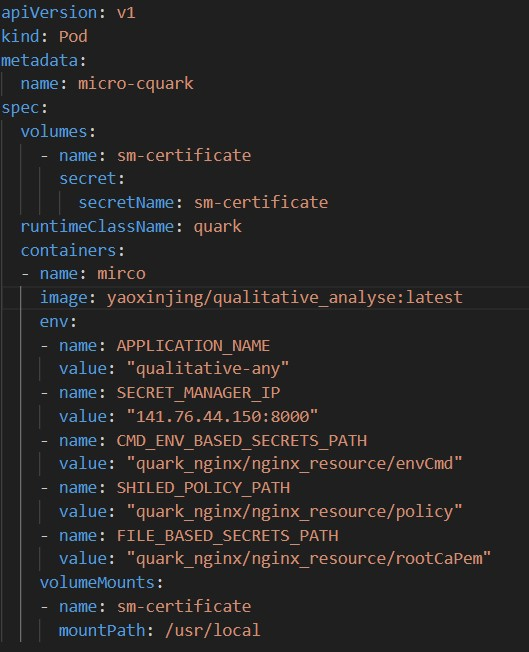
\includegraphics[height=0.3\textheight]{images/cquark_deploy_yaml.jpg}
    \caption[YAML configuration file for deploying an application in confidential Quark]{YAML configuration file for deploying an application in confidential Quark}
    \label{fig:cquark_deploy_yaml}
\end{figure}

Confidential Quark deploys the application using the YAML configuration file shown in Figure~\ref{fig:cquark_deploy_yaml}. The new application deployment scheme and the YAML configuration file are explained in Section~\ref{sec:secure_application_deployment}. 
Figure~\ref{fig:analysis_Secure_Application_Deployment} (b) outlines the steps and outcomes of the application deployment process in the confidential Quark environment.

Figure~\ref{fig:analysis_Secure_Application_Deployment} (a) shows that the \acrshort{CVM} successfully attests its identity to the secret manager during the remote attestation and provisioning. Currently, the secret manager operates in \texttt{native} mode, verifying the consistency 
between the shield startup hash and the reference hash \emph{shield\_startup\_ref\_measurement} specified in the shield policy (Figure~\ref{fig:generic_policy}). The shield startup hash includes the measurement for binaries and shared libraries loaded during application setup, 
Qkernel configuration files, etc. (refer to Section~\ref{sec:Enclave_Runtime_Measurement}). As depicted in Figure~\ref{fig:analysis_Secure_Application_Deployment} (b), the \acrshort{CVM} successfully retrieves the secret from the secret manager and prints them. 
It's worth noting that the directory \texttt{/secret} remains invisible from the host (as seen in Figure~\ref{fig:analysis_Secure_Application_Deployment} (c)), as file type secrets and the filesystem mounted under the \texttt{/secret} directory are within the \acrshort{CVM}. 
Therefore, the security issue~\ref{vulnerability:1} and ~\ref{vulnerabilities:6} (b) of OCI runtime interface~\cite*{oci-runtime-spec} summarized in Section~\ref{sec:security_analyse_oci_summary} have been effectively resolved.


\begin{figure}[!htb]
    \subfloat[Secret manager succesfully autheticates \acrshort{CVM}'s state during remote attestation\label{fig:cquark_kbs_start}]{%
    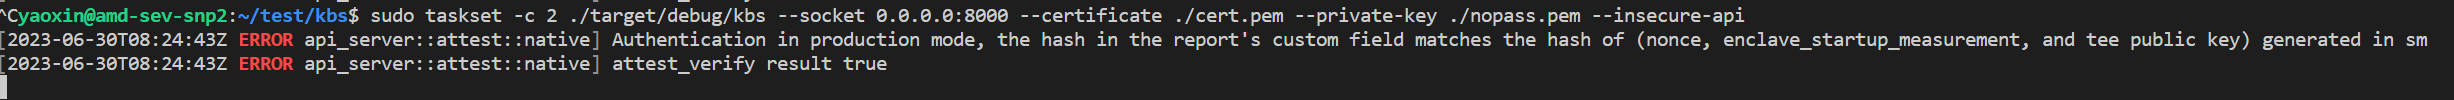
\includegraphics[clip,width=\columnwidth]{images/cquark_kbs_start.PNG}%
  }

    \subfloat[Application deployment process\label{fig:cquark_deployment_result}]{%
      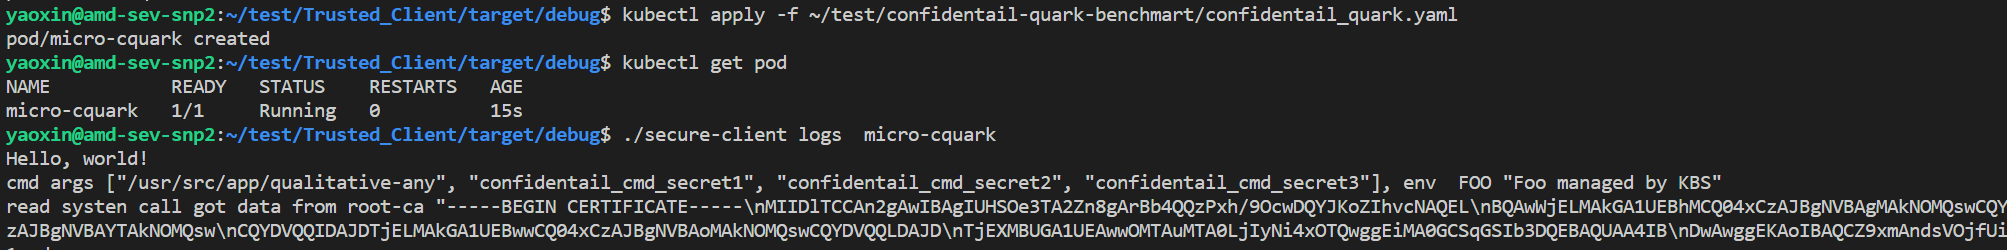
\includegraphics[clip,width=\columnwidth]{images/cquark_deployment_result.PNG}%
    }
    
    \subfloat[File type secrets under directory \textbf{/secret} are invisible on the host\label{fig:cquark_deployment_result_file_secret_mount_location}]{%
      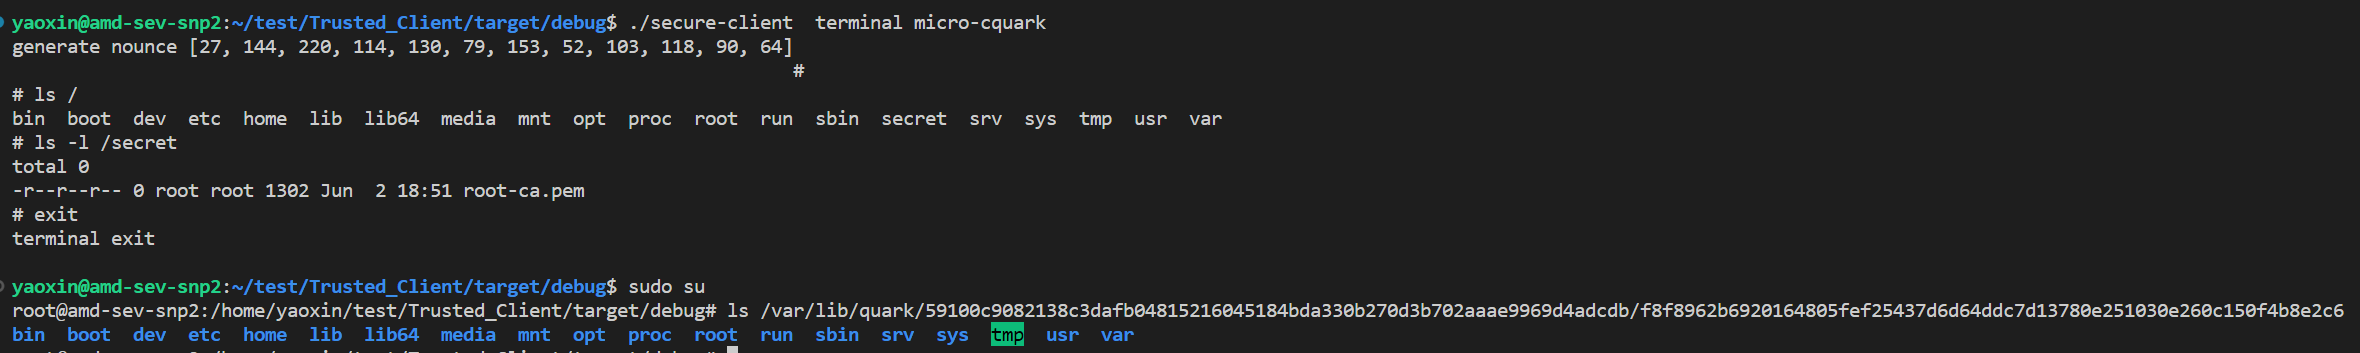
\includegraphics[clip,width=\columnwidth]{images/cquark_deployment_result_file_secret_mount_location.png}%
    }
    
    \caption[The result for secure application deployment in confidential Quark]{The result for secure application deployment in confidential Quark.\label{fig:cquark_deployment}}
    \label{fig:analysis_Secure_Application_Deployment}
\end{figure}


\subsection{Authentication and Access Control for EXEC Requests}
\label{sec:eva_qualitativ_secure_exec}
Section~\ref*{sec:design_EXEC_Requests} proposes a novel schema for handling EXEC requests. As depicted in Figure~\ref{fig:cquark_cmd_exec} (a), both privileged and unprivileged users are prohibited from executing the \texttt{ls /} command within the \acrshort{CVM} due to the shield policy's restriction on 
running commands in the root directory. 
\begin{figure}[!b]

  \subfloat[The shield rejects the privileged and non-privileged command \texttt{ls /}\label{fig:ls_exec}]{%
  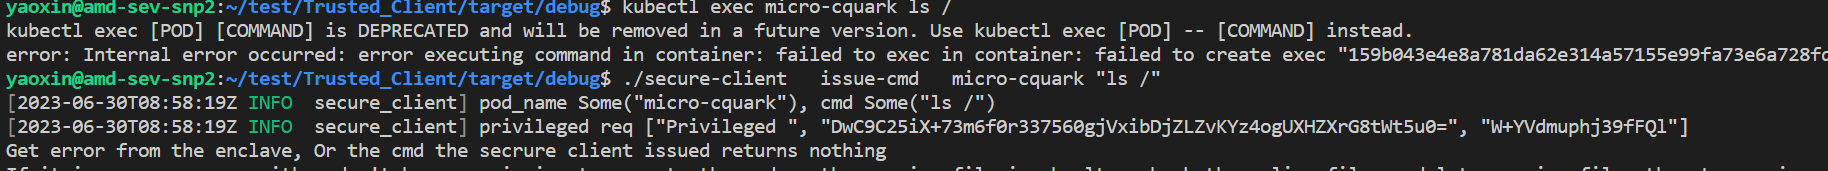
\includegraphics[clip,width=\columnwidth]{images/ls_exec.png}%
  }

  \subfloat[Issuing unprivileged command \texttt{ls /var/log}\label{fig:ls_allow_unprivileged}]{%
  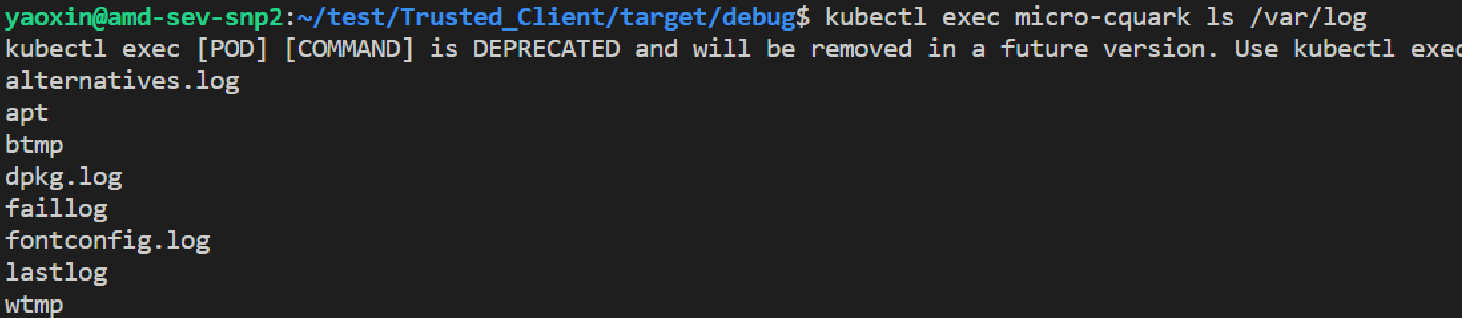
\includegraphics[clip,width=\columnwidth]{images/ls_allow_unprivileged.png}%
  }

  \subfloat[Issuing privileged command \texttt{ls /var/}\label{fig:ls_allow_previleged}]{%
    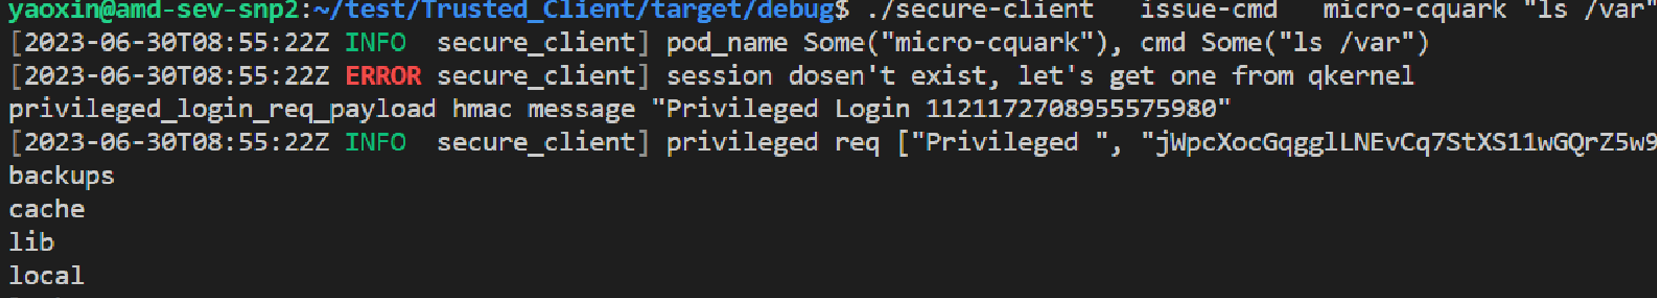
\includegraphics[clip,width=\columnwidth]{images/ls_allow_previleged.png}%
  }
  
  \subfloat[Issuing privileged command \texttt{cat} ]{%
  \label{fig:cat_pri}
    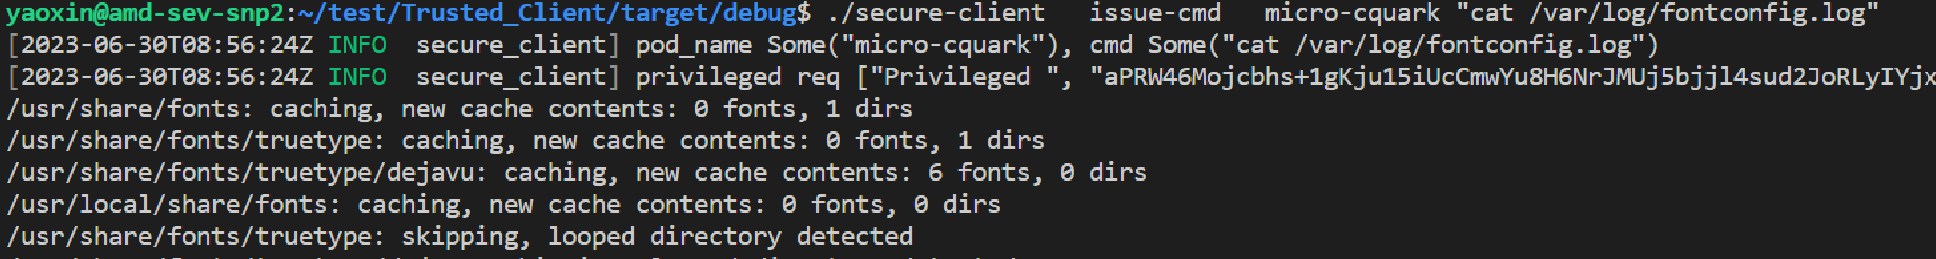
\includegraphics[clip,width=\columnwidth]{images/cat_pri.png}%
  }

  \subfloat[Issuing unprivileged command \texttt{cat}]{%
  \label{fig:cat_unpri}
  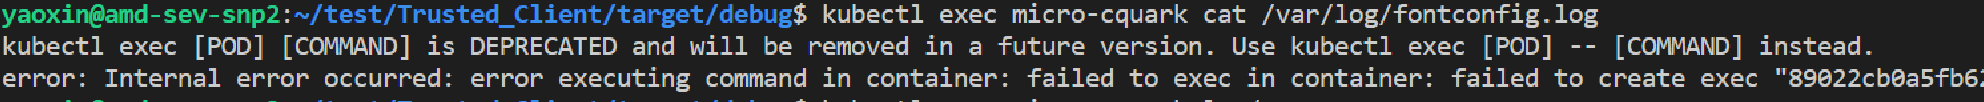
\includegraphics[clip,width=\columnwidth]{images/cat_unpri.png}%
}

\subfloat[Attempting to allocate a terminal through both \emph{securectl} and \emph{kubectl}\label{fig:cquark_terminal}]{%
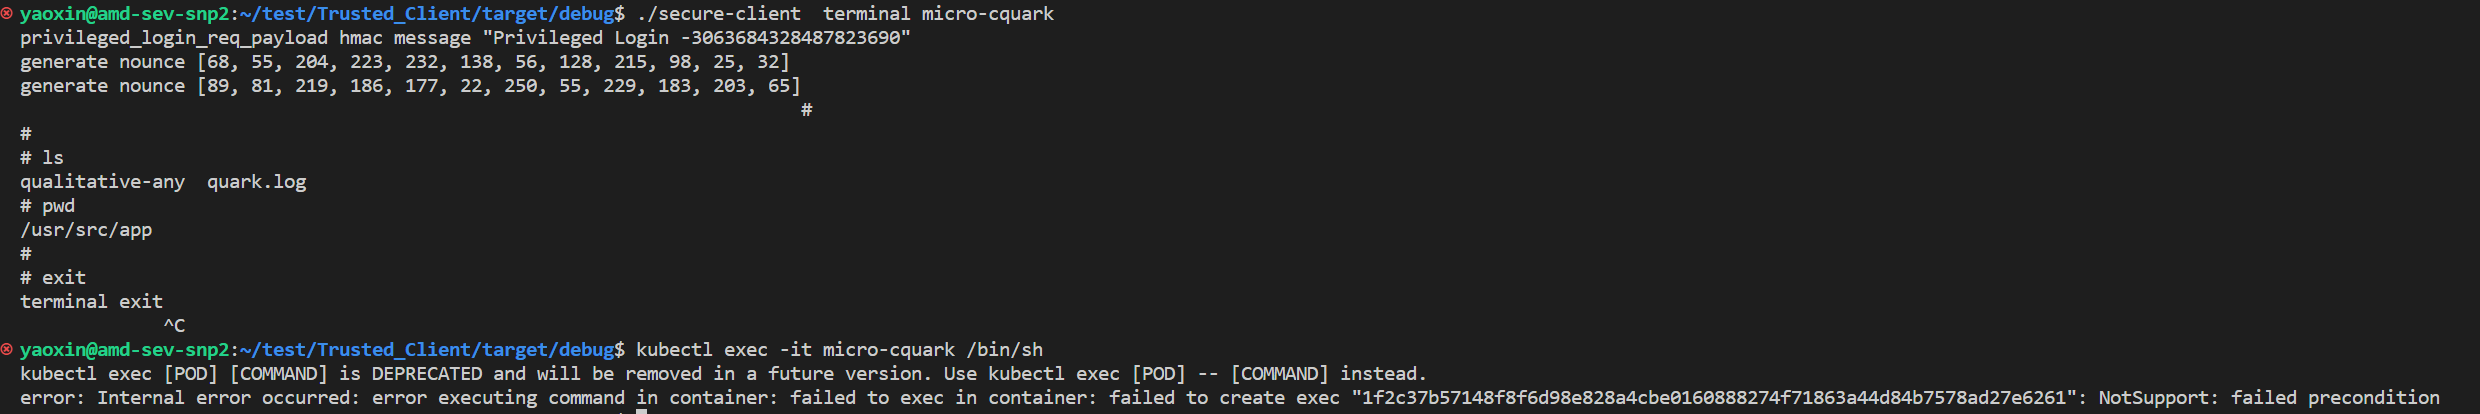
\includegraphics[clip,width=\columnwidth]{images/cquark_terminal.png}%
}

\subfloat[The privileged request is denied as the session is old\label{fig:seesion_is_old}]{%
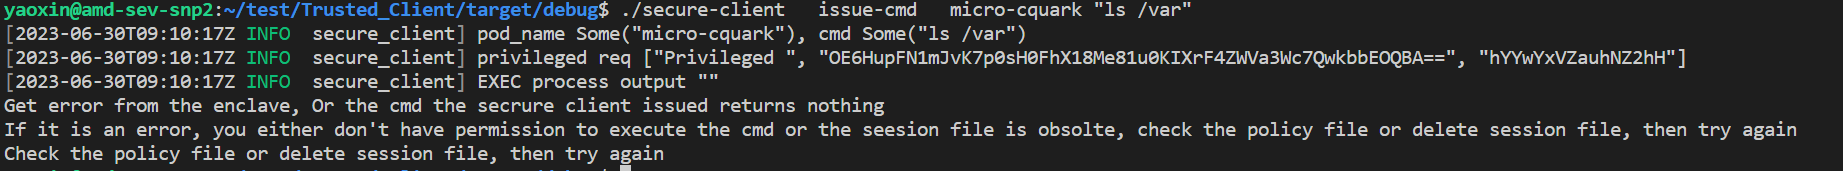
\includegraphics[clip,width=\columnwidth]{images/seesion_is_old.PNG}%
}
  
  \caption[The result of issuing commands to the application in confidential Quark]{The result of issuing  commands to the application in confidential Quark\label{fig:exec}}
  \label{fig:cquark_cmd_exec}

\end{figure}
Figure~\ref{fig:cquark_cmd_exec} (b) and~\ref{fig:cquark_cmd_exec} (c) illustrates that unprivileged and privileged users can issue the \texttt{ls /var/log} and \texttt{ls /var}  commands to the application, respectively. 
This allowance stems from the shield policy's command and directory allowlist, which includes these specific commands and their corresponding arguments. Conversely, since the command whitelist for non-privileged users excludes the \texttt{cat} command, unprivileged users are incapable of issuing the \texttt{cat} command to 
access the log file \texttt{/var/log/fontconfig.log} (figure~\ref{fig:cquark_cmd_exec} (e)). Furthermore, as Figure~\ref{fig:cquark_cmd_exec} (f) shows, privileged users can spawn a terminal, while unprivileged users cannot. 
This is as expected since the unprivileged user's command allowlist does not include any terminal allocation instructions. Besides, \emph{securectl} saves the session id and counter as a file locally and uses this file to build the frame structure for privileged commands. Compared to Figure~\ref{fig:cquark_cmd_exec} (c), the same 
privilege command is denied in Figure~\ref{fig:cquark_cmd_exec} (g) as the session id in the file is modified to a number that the shield does not know. This shows that the shield can prevent reply attacks from EXEC requests. 




In addition, the \emph{securectl} is modified to print the command and the command execution result. As shown in Figure~\ref{fig:cquark_priviled_cmd_result_protection}, both the EXEC command and its execution result are cryptographically protected. The protection mechanisms for the command 
and the execution result are discussed in Sections~\ref{sec:design_prptect_privileged_request} and~\ref{sec:design_STDIO_PROTECTION}, respectively.
\begin{figure}[!htb]
  \centering
  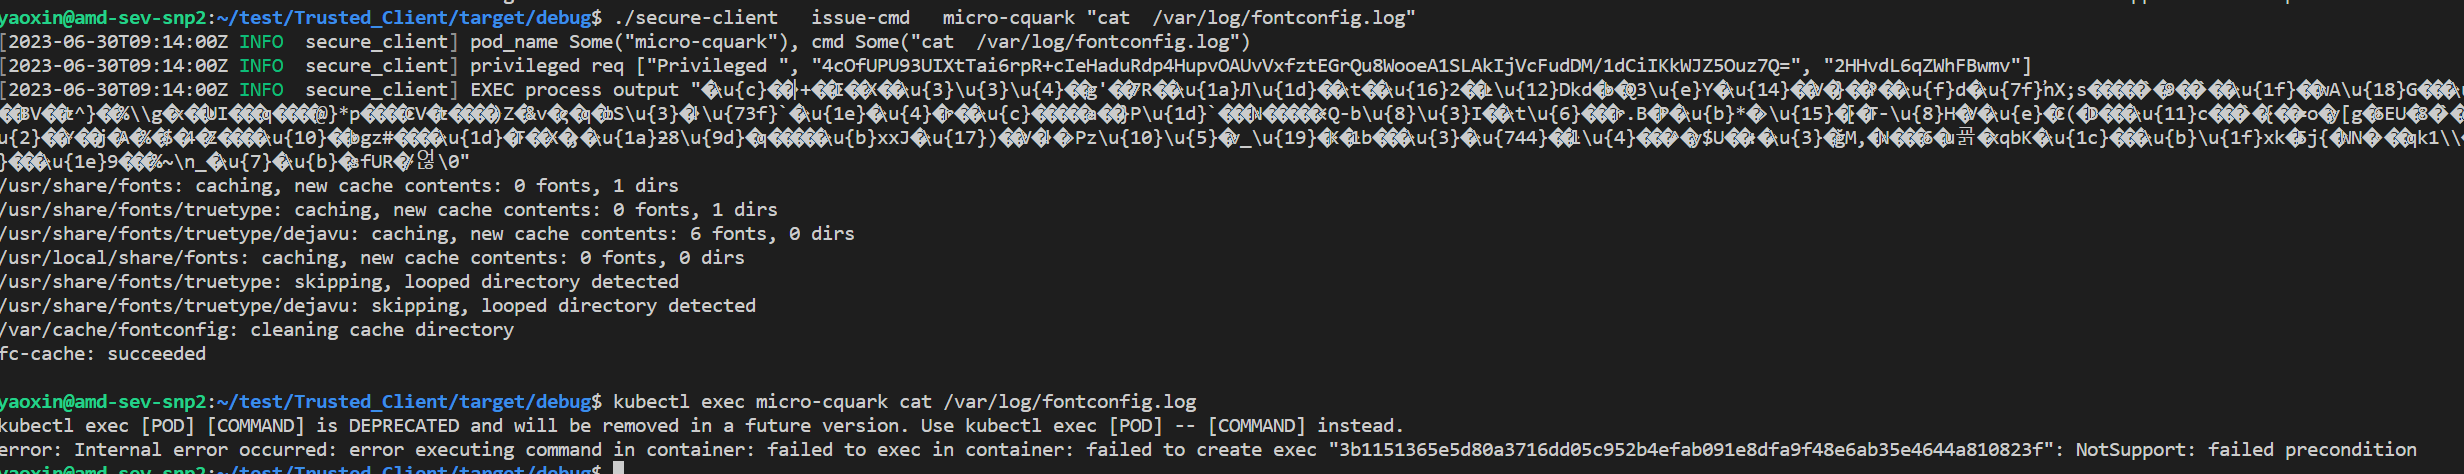
\includegraphics[width=1\textwidth]{images/cquark_priviled_cmd_result_protection.PNG}
  \caption[The privileged command and its execution result are encrypted]{The privileged command and its execution result are encrypted}
  \label{fig:cquark_priviled_cmd_result_protection}
\end{figure}

The above examples demonstrate that the vulnerability~\ref{vulnerabilities:3} of the OCI runtime interface~\cite*{oci-runtime-spec} summarized in Section~\ref{sec:security_analyse_oci_summary} can be effectively addressed.



\subsection{Guest User Space Process's STDIO Protection}
\label{sec:eva_qualitativ_secure_stdio}
The program~\cite*{qualitativ_programs} used in qualitative analysis is non-interactive. Since the option \emph{no\_interactive\_process\_stdout\_err\_encryption} in the policy is true, the shield will encrypt STDOUT and STDERR for privilege-level processes. Thus, only privileged users, 
namely the application owners, can view the logs using \emph{securectl} (as shown in Figure~\ref{fig:qualitativ_non_interactive_process_stdio} (a)). On the other hand, non-privileged users who use the command \emph{kubectl log} can only access the logs in ciphertext (Figure~\ref{fig:qualitativ_non_interactive_process_stdio} (b)).
Furthermore, Figure~\ref{fig:cquark_priviled_cmd_result_protection} showcases that the execution results of privilege-level commands are also encrypted.

\begin{figure}[!htb]

  \subfloat[Accessing application log using \emph{securectl}\label{fig:cquark_log_from_secure_ctl}]{%
    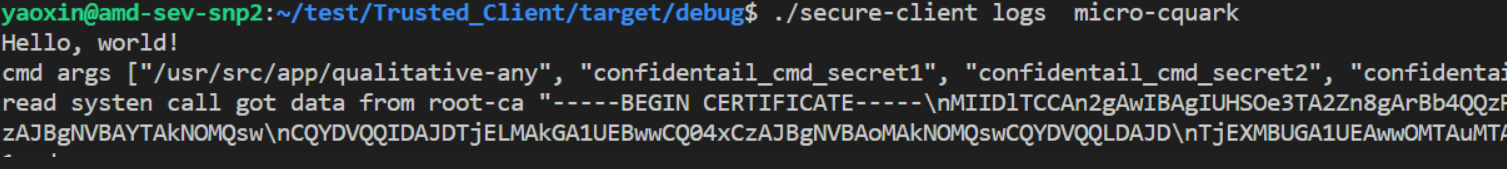
\includegraphics[clip,width=\columnwidth]{images/cquark_log_from_secure_ctl.png}%
  }
  
  \subfloat[Accessing application log using \emph{kubectl}\label{fig:cquark_log_from_kubectl}]{%
    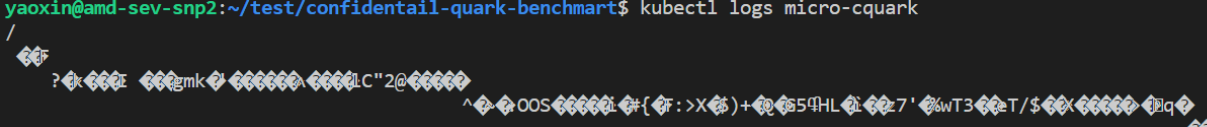
\includegraphics[clip,width=\columnwidth]{images/cquark_log_from_kubectl.png}%
  }
  
  \caption[Accessing non-interactive application log through kubectl and securectl]{Accessing non-interactive application log through kubectl and securectl}
  \label{fig:qualitativ_non_interactive_process_stdio}
\end{figure}



In the case of interactive applications, the busybox is used as an example. The corresponding YAML file for deployment can be found in commit~\cite*{artifacts_busybox}. Since protecting the terminal's STDIO is out of the scope,  the STDIO shield 
only encrypt the STDOUT and STDERR outputs for the interactive application process in the same way that it encrypts the STDOUT and STDERR outputs of the non-interactive process.
\begin{figure}[!htb]

  \subfloat[Attaching to application using \emph{kubectl -it attach}\label{fig:attach_failed}]{%
  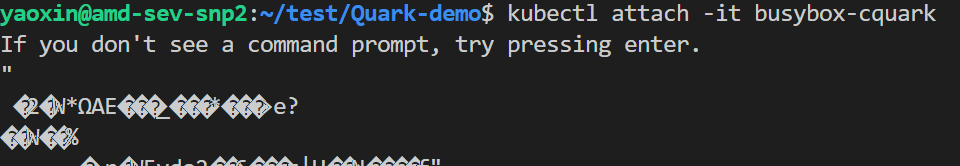
\includegraphics[clip,width=\columnwidth]{images/attach_failed.png}%
}

\subfloat[Accessing application log using \emph{kubectl}\label{fig:interactive_log}]{%
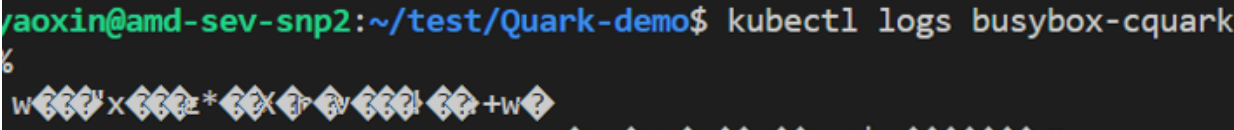
\includegraphics[clip,width=\columnwidth]{images/interactive_log.png}%
}

  \caption[Accessing logs and attaching to an interactive application ]{Accessing logs and attaching to an interactive application}
  \label{fig:qualitativ_interactive_process_stdio}
\end{figure}
The demo set \emph{interactive\_porcess\_stdout\_err\_encryption} option in the policy to true. Therefore, as shown in Figure~\ref{fig:qualitativ_interactive_process_stdio} (a),  a non-privileged user can attach a terminal to the application. However, the terminal functionality is limited as the application only returns 
ciphertexts. Furthermore, the logs generated by the application are also encrypted (Figure~\ref{fig:qualitativ_interactive_process_stdio} (b)). 


These examples showcase that STDIO shield can protect the STDOUT and STDERR of processes running in CVM, thereby partially mitigating vulnerability~\ref{vulnerabilities:2} of the OCI runtime interface~\cite*{oci-runtime-spec} summarized in Section~\ref{sec:security_analyse_oci_summary}. 
The protection for the STDIO of interactive processes (i.e., terminal) is left for future implementation.


\subsection{Qkernel Log Management}
\label{sec:eva_qualitativ_secure_log}
In vanilla Quark, the logs generated by Qvsivor and Qkernel are kept in the same file, namely \texttt{/var/log/quark/quark.log}. In order to differentiate the logs,  the logs generated by Qkernel are prefixed with the keyword \texttt{Qkernel} (Figure~\ref{fig:quark_qkernel_log} (a)).
\begin{figure}[!htb]

    \subfloat[Vanilla Quark\label{fig:vanilla_qkernel_Log}]{%
    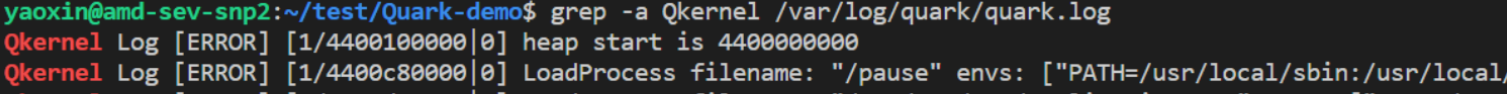
\includegraphics[clip,width=\columnwidth]{images/vanilla_qkernel_Log.png}%
  }

  \subfloat[Confidential Quark\label{fig:cquark_qkernel_log}]{%
  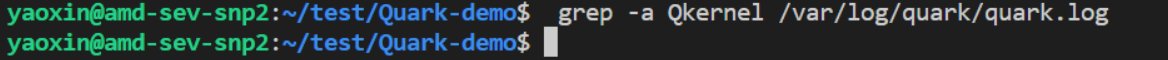
\includegraphics[clip,width=\columnwidth]{images/cquark_qkernel_log.png}%
}
  
    \caption[Accessing guest kernel log in confidential and vanilla Quark]{Accessing guest kernel log in confidential and vanilla Quark}
    \label{fig:quark_qkernel_log}
\end{figure}


In confidential Quark, the Qlog manager's max log level is set to \texttt{OFF}. Therefore, the guest kernel logging system does not print logs to the host (Figure~\ref{fig:quark_qkernel_log} (b)).

\subsection{Qkernel Guest System Call Interception}
\label{sec:eva_qualitativ_secure_syscall}
\begin{figure}[!htb]
    \centering
    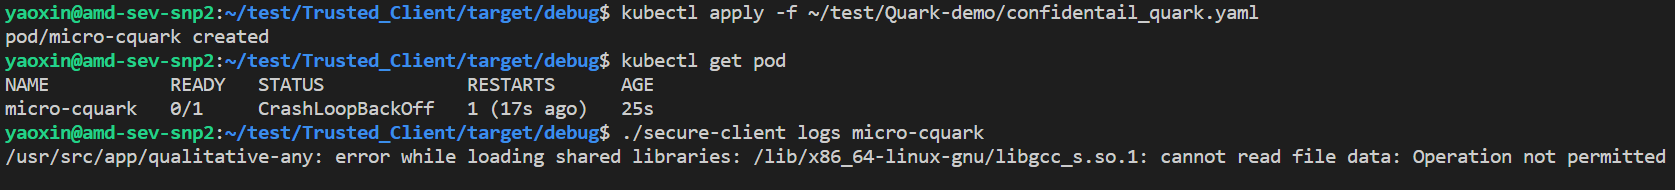
\includegraphics[width=1\textwidth]{images/application_failed_to_start_due_to_syscall_interceptor.png}
    \caption[Failed to run an application when the read system call is excluded from the system call interceptor's allowed list]{Failed to run an application when the read system call is excluded from the system call interceptor's allowed list}
    \label{fig:application_failed_to_start_due_to_syscall_interceptor}
\end{figure}


Figure ~\ref{fig:application_failed_to_start_due_to_syscall_interceptor} presents a demo of the guest interceptor. By removing the read system call ID from the system call allowlist in the shield policy shown in Figure~\ref{fig:generic_policy}, 
the application process failed to start. The failure occurred because it lacked permission to execute the read system call for loading dynamic libraries.

\subsection{Application Runtime Measurements}
\label{sec:eva_qualitativ_runtime_meausre}
According to the discussion in Section~\ref{sec:Enclave_Runtime_Measurement}, the shield measures the binaries (e.g., shared libraries, command binaries) loaded from the host at application runtime and compares the resulting hashes with the reference hashes in the shield policy.  

Figure~\ref{fig:cquark_runtime_runtime_lib_measurement_demo} shows a measurement demo of the shared library. Regarding the setup, the reference hash of the library \texttt{/lib/x86\_64-linux-gnu/libgcc\_s.so.1} in the shield policy is intentionally set to empty and the maximum logging level of the 
Qlog manager is configured to \texttt{Debug}. Next, the modified policy is deployed to the secret manager. The Qkernel logs in Figure~\ref{fig:cquark_runtime_runtime_lib_measurement_demo} show that the \acrshort{CVM} encountered a crash due to a discrepancy between the measurements of the loaded library and the corresponding reference hash stored in the policy.


\begin{figure}[!htb]
    \centering
    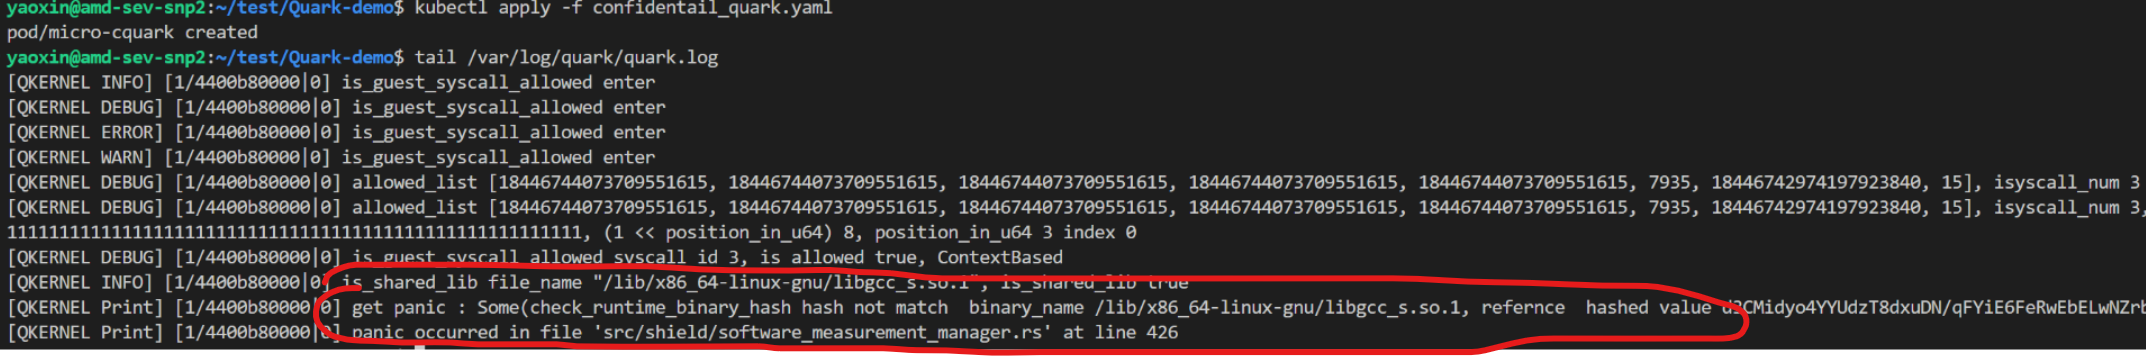
\includegraphics[width=1\textwidth]{images/cquark_runtime_runtime_lib_measurement_demo.png}
    \caption[Shared library measurement demo]{Shared library measurement demo}
    \label{fig:cquark_runtime_runtime_lib_measurement_demo}
\end{figure}


To demonstrate measuring the executable loaded during application runtime, the shield policy is modified to set the reference hash for the \texttt{ls} binary to empty and the Qlog manager's max log level to \texttt{Info}. Then, the \emph{kubectl} is used to 
issue the command \texttt{ls /var/log} to the application. Figure~\ref{fig:cquark_runtime_runtime_binary_measurement_demo} shows that the command failed to get a response. As can be seen from the Qkernel logs, the reason for the Qkernel crash is a mismatch between the 
reference hash of the \texttt{ls} binary and its actual hash.


\begin{figure}[!htb]
    \centering
    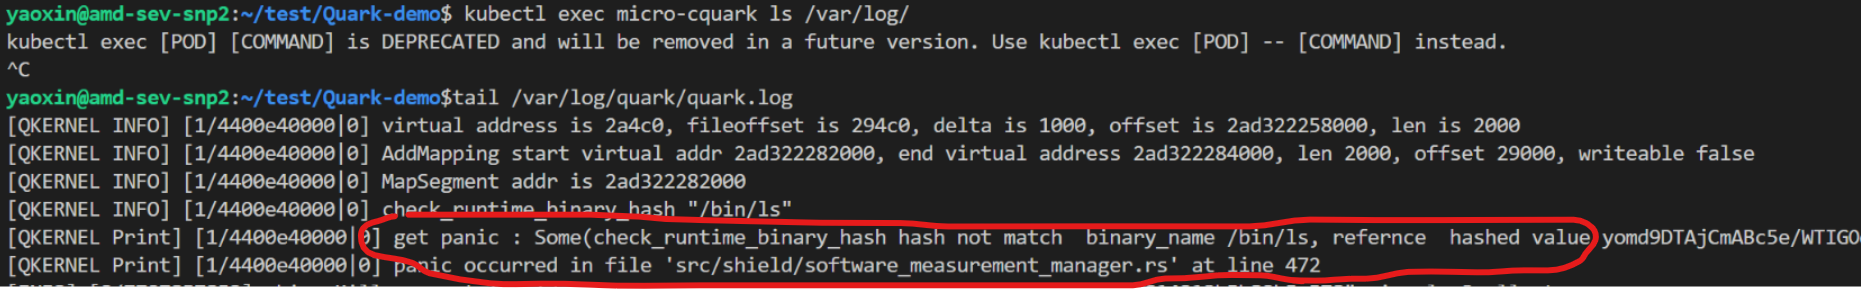
\includegraphics[width=1\textwidth]{images/cquark_runtime_runtime_binary_measurement_demo.png}
    \caption[Runtime binary measurement demo]{Runtime binary measurement demo}
    \label{fig:cquark_runtime_runtime_binary_measurement_demo}
\end{figure}



As discussed in Section~\ref{sec:Enclave_Runtime_Measurement}, the shield will measure the binaries and shared libraries during the application restart process and compare the resulting measurement, known as application restart hash, with the application startup reference hash. 
Figure~\ref{fig:cquark_application_restart_demo} (a) exemplifies this process.
\begin{figure}[!htb]
    \subfloat[Application restart workflow\label{fig:app_restart_eva}]{%
    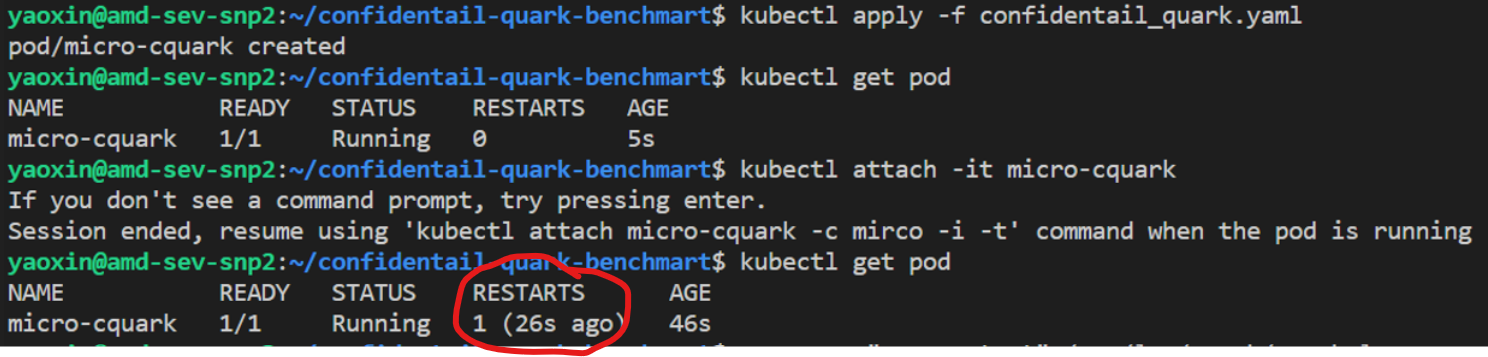
\includegraphics[clip,width=\columnwidth]{images/app_restart_eva.png}%
  }

  \subfloat[Qkernel log\label{fig:app_restart_result}]{%
  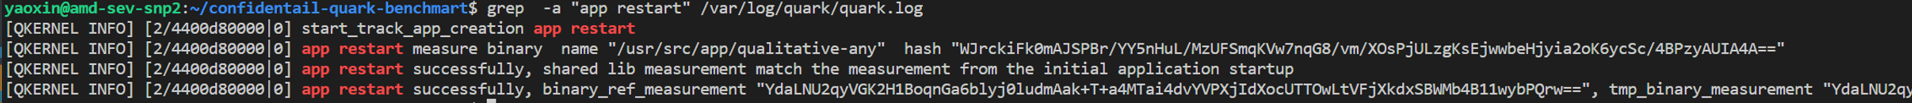
\includegraphics[clip,width=\columnwidth]{images/app_restart_result.png}%
  }
  
    \caption[Demo for  administration to application restart]{Demo for administration to application restart}
    \label{fig:cquark_application_restart_demo}
\end{figure}

In this example, the Qlog manager’s max log level is configured to \texttt{Info} and the keywords \texttt{stdin: true} and \texttt{tty: true} are added to the container spec of the YAML file used to deploy the 
application (Figure~\ref{fig:cquark_deployment}). These keywords keep the application’s stdin open and notify Kubernetes\cite*{k8s} that it should be regarded as a terminal. As shown in Figure~\ref{fig:cquark_application_restart_demo} (a), the application is first created using the modified YAML file. Once the application starts, \emph{kubectl attach -it} is used to 
attach to the application process and send \texttt{ctrl c} to the process. The \texttt{ctrl c} will cause the terminal IO redirection thread sends \texttt{SIGINT} to terminate the application, as discussed in section~\ref{sec:security_analyse_STDIO}. The output of the second \emph{kubectl get} command confirmed that the application had successfully restarted. 
As can be seen from the Qkernel logs shown in Figure~\ref{fig:cquark_application_restart_demo} (b), the shield measured binaries and shared libraries loaded from the host during the application restart. The shield compared the resulting measurements with the application startup reference hash to determine that the binaries and shared libraries loaded during 
the two startups were consistent.


The above three examples highlighted the ability of the shield to refuse execution when an adversary tries to trick the \acrshort{CVM} into loading harmful code during application runtime and restart. 


\subsection{Summary of Qualitative Analysis}
\label{sec:eva_qualitativ_summary}




This section showcased that the system implemented in Chapter~\ref{sec:implementation} could mitigate most vulnerabilities of the OCI runtime interface summarized in Subsection~\ref{sec:security_analyse_oci_summary}. Table~\ref{tab:eva_qualitativ_summary} provides a concise overview of 
these vulnerabilities, as well as their respective mitigations and corresponding demonstration location.

Subsection~\ref{sec:eva_qualitativ_secure_depl} demonstrated that vulnerability 1 in Table~\ref{tab:eva_qualitativ_summary} is successfully mitigated by offloading secret management and deployment to the secret manager and shield. In relation to vulnerability 2, 
Subsection~\ref{sec:eva_qualitativ_secure_stdio} revealed the STDIO shield's capability to encrypt the STDOUT and STDERR of guest processes, thereby safeguarding the application's logs and execution results of privileged commands. Besides, it is important to note that the STDIO 
shield does not extend its protection to the terminal (out of the scope). Thus, an attacker can use \emph{kubectl attach} to connect to an interactive application's STDIO and send arbitrary commands. Although the execution results of these commands remain encrypted, 
the attacker can, for example, deletes the application's confidential data. 


The demo in Subsection~\ref{sec:eva_qualitativ_secure_exec} proved that the shield can perform access control and authentication on EXEC requests. Moreover, as depicted in Figure~\ref{fig:cquark_priviled_cmd_result_protection} of the same subsection, privileged commands are encrypted. 
To this end, vulnerability 3 in Table~\ref{tab:eva_qualitativ_summary} is resolved. It is important to note that vulnerability 4 (a) is not addressed, as it falls outside the scope of the thesis. 

For vulnerability 4 (b), Figure~\ref{fig:analysis_Secure_Application_Deployment} (a) in Subsection~\ref{sec:eva_qualitativ_secure_depl} showed that the secret manager could guarantee the integrity of binaries and shared libraries loaded before the application process is launched. 
This is done by verifying the shield startup hash embedded in the attestation report. Subsection~\ref{sec:eva_qualitativ_runtime_meausre} further demonstrated that the shield could ensure the integrity of binaries and shared libraries loaded during application runtime and restart. 
Additionally, Subsection~\ref{sec:eva_qualitativ_secure_syscall} showcased that the system calls interceptor rejects read system calls based on the shield policy. The design of the system interceptor can be found in Section~\ref{sec:design_Interceptor}. It successfully mitigates vulnerability 5. 



Finally, concerning vulnerability 6, Subsection~\ref{sec:eva_qualitativ_secure_log} confirmed the capability of the Qkernel log manager for administrating the VM's logs. Figure~\ref{fig:analysis_Secure_Application_Deployment} (a) in Subsection~\ref{sec:eva_qualitativ_secure_depl} then showed 
that the integrity of the guest kernel startup parameter could be ensured since it is part of the shield startup hash, which is verified by the secret manager during remote attestation. Besides, the guest kernel (Qkernel)  binary should be measured by the TEE during VM 
setup and sent to the secret manager as the VM boot measurement in the attestation report for integrity checking. However, due to the lack of TEE support for Quark, the secret manager receives a simulated report containing a dummy VM boot measurement. Consequently, 
the secret manager cannot verify the integrity of the Qkernel binary. Vulnerability 6 is, therefore, only partially mitigated. 


\begin{table}[H]
  \centering%
  \setlength{\tabcolsep}{4pt}
  \caption{Vulnerabilities of OCI runtime interface in the confidential computing and suggested solutions\label{tab:eva_qualitativ_summary}}
  \footnotesize
  \resizebox*{1\columnwidth}{!}{
  \begin{tabularx}{\linewidth}{@{}l>{\RaggedRight}X>{\RaggedRight}X%
    >{\RaggedRight}I}% The target layout does not centre the text so we don't want \centering
    \toprule% nicer rules courtesy of booktabs - but then we need to drop the verticals
      & \thead{Vulnerabilities} & \thead{Solution} & \multicolumn{1}{c}{\small \bfseries Comment}%
    \tabularnewline\midrule%
    \textbf{1} &Secrets are managed and deployed by k8s and runtime&
    Offload the secret management and deployment to the secret manager and the shield
    
    % \begin{itemize}
    % \item I would like this text to be bulleted with ragged right. I would also like this text to be bulleted with ragged right.
    % \item I would also like this text to be bulleted with ragged right.
    % \item I would also like this text to be bulleted with ragged right.
    % \end{itemize}
    &
    \item Vulnerability resolved.
    \item A demo can be found in section~\ref{sec:eva_qualitativ_secure_depl}.

    % \item I would also like this text to be bulleted with ragged right.
    % \item I would also like this text to be bulleted with ragged right.
    \tabularnewline
    \addlinespace\midrule%
    \textbf{2} & Lack of protection for processes' STDIO
    & Add STDIO shield in Qkernel
    &  
    \item Vulnerability partially resolved.
    \item STDIO shield only encrypts STDOUT and STDERR (Demo in Section~\ref{sec:eva_qualitativ_secure_stdio})
    \item Protection for STDIO of interactive processes (i.e., terminal) is out of the scope 
    

    \tabularnewline
    \addlinespace\midrule%
    \textbf{3} &EXEC operation
    \begin{enumerate}[label=(\alph*), align=left, left=0pt, itemsep=1pt]
        \item Missing authentication and access control
        \item Commands are transmitted by untrusted runtime 
    \end{enumerate}
    & 
    \begin{itemize}[]
      \item Add EXEC checker in Qkernel.
      \item Apply end-to-end encryption for privileged commands.
    \end{itemize}
      
    &  
    \item Vulnerability resolved.
    \item A demo can be found in section~\ref{sec:eva_qualitativ_secure_exec}.


    \tabularnewline  
    \addlinespace\midrule%
    \textbf{4(a)} & Lack of protection for data written to volume
    & Add filesystem shield.
    &  
    \item Out of the scope.
    

    \tabularnewline
    \addlinespace\midrule%
    \textbf{4(b)} & Loading compromised binary and share library
    & 
    \begin{itemize}[]
      \item Measure binaries and shared libraries using the software measurement manager.
      \item Verify the measurement results against the reference hashes in the shield policy.
    \end{itemize}
    &
    \item Vulnerability resolved
    \item Demo can be found in sections~\ref{sec:eva_qualitativ_secure_depl} and~\ref{sec:eva_qualitativ_runtime_meausre}.
    

    \tabularnewline
    \addlinespace\midrule%
    \textbf{5} & Seccompe-based system call interception is not suitable for confidential computing
    & Add guest system call interceptor&
    \item Vulnerability resolved
    \item Demo can be found in section~\ref{sec:eva_qualitativ_secure_syscall}.
    

    \tabularnewline
    \addlinespace\midrule%
    \textbf{6} & Lack of mechanism to ensure the proper configuration of the container running environment.
    \begin{enumerate}[label=(\alph*), align=left, left=0pt, itemsep=1pt]
      \item The integrity of guest kernel binary and guest kernel startup parameters.
      \item The proper configuration of the guest logger.
    \end{enumerate}
    & 
    \begin{itemize}[]
      \item Use Qkernel log manager to administrate the guest logs.
      \item Employ the secret manager to verify the integrity of the guest kernel binary and guest kernel parameters. 
    \end{itemize}
    &
    \item Vulnerability partially resolved.
    \item Demo can be found in section~\ref{sec:eva_qualitativ_secure_depl} and~\ref{sec:eva_qualitativ_secure_log}.
    \item The secret manager cannot verify the integrity of the Qkernel binary because the binary should be measured by TEE, which is not yet supported by Quark (Out of scope).
    \tabularnewline
    \bottomrule
\end{tabularx}}
\end{table}







\section{Quantitative Analysis}
\label{sec:eva_Quantitative}
This section evaluates the performance of the system implemented in Chapter~\ref{sec:implementation} in terms of both latency and throughput.

\subsection{Overview of Quantitative Analysis}
\label{sec:eva_overwiwe_Quantitative}

The quantitative analysis evaluates the performance of the system implementation in terms of both latency and throughput. It includes variant micro and macro benchmarks. Microbenchmarks are performed to understand the latency overhead introduced by individual components in the shielding layer, while macro benchmarks aim to evaluate the 
performance loss of running real-world applications in confidential Quark. The section is structured around the following subsections. 

Subsection~\ref{Hardware_and_Software_Setup} first describes the hardware and software setup for benchmarking. Subsection~\ref{Attestation_Report_Syscall} then evaluates the speed of obtaining three types of attestation reports using a microbenchmark. Subsequently, the latency overhead of the guest system 
call interceptor is evaluated in Subsection~\ref{bench_Interceptor}. Unlike vanilla Quark, confidential Quark stores file-type secrets in the guest's memory. Therefore, Subsection~\ref{bench_reading_file_secret} estimates the speed at which applications can access file-type secrets in vanilla and confidential Quark.
 
Later, in Subsection~\ref{bench_issuing_Instructions}, the latency benchmark results for issuing commands using \emph{kubectl} in confidential and vanilla Quark are presented. Also, the speed of sending the same commands in confidential Quark using \emph{kubectl} and \emph{securectl} is compared. Then after 
estimating the performance of accessing binary-mapped memory regions in Subsection~\ref{accesiing_binary_mapped_memory}. Subsection~\ref{micro_app_start_up} then observes the effect of the number of file type secrets and the size of the measured binary on the application startup time duration.


In Subsection~\ref{macri_app_start_up},  a macro-benchmark using Nginx~\cite*{nginx} and Redis~\cite*{redis} are performed. The benchmark explores the performance differences between applications running in confidential and vanilla Quark regarding startup time, exit time, and throughput. Furthermore, the Redis benchmark~\cite*{Redis_benchmark} and the 
Apache HTTP server benchmarking tool~\cite*{ab} are utilized to measure application throughput. Subsection~\ref{tcb} analyzes the TCB overhead incurred by the shield and compares the TCB sizes of Kata containers~\cite*{Kata-Containers} and confidential Quark.  

A summary of the quantitative analysis can be found in Subsection~\ref{sec:qualitativ_sum}.



\subsection{Hardware and Software Setup}\label{Hardware_and_Software_Setup}

This subsection summarizes the hardware and software settings utilized for the benchmarks. Regarding hardware, all measurements are performed on a server with AMD EPYC 7443P 24-Core CPU and 4 DDR4-3200 Mhz-16GB RAM. Regarding software, the host OS is Ubuntu 20.04.6 LTS and Linux 5.19.0 kernel. 
Furthermore, the CPU governor is set to performance mode, and Hyper-Threading and Turbo Boost are disabled to establish a low-noise environment for benchmarking with reproducible results. Besides, all test binaries (e.g., Qvisor, Qkernel) are built in 
release mode. Unless otherwise mentioned, the vanilla Quark's version is v0.2.0, and confidential Quark uses this commit~\cite*{qualitativ_confidentail_quark}.


Regarding the tools for measuring latency, since all benchmark objects are located in the guest, the guest system call \emph{clock\_gettime(monotonic)}~\cite*{clock_gettime} is used for time measurement, and the results are printed to the host using the Qkernel logging system. The 
benchmarking framework~\cite*{benchamark_framework} can analyze the results by parsing the Quark log under the host directory \texttt{/var/log/Quark}. In addition, all benchmarks are performed multiple times. The following subsections illustrate the measurement results in average time and variance format.

\subsection{Micro-benchmark – Attestation Report Syscall}
\label{Attestation_Report_Syscall}

Confidential Quark enables applications to obtain three types of attestation reports via a system call. The type of the report includes simulated AMD SEV-SNP report, software reports signed by secret manager's key, or software reports signed by the application. This subsection assesses the speed with which the 
application acquires various reports. For this purpose, a Rust microbenchmark\cite*{benchamark_Attestation_Report_Syscall} is prepared. In order to ensure stable results, the test program submitted 10,000 requests for each type of report to the Qkernel. The benchmark program is containerized, 
and the YAML file for the deployment can be found in the repository~\cite*{perf_test_repo}.

\begin{figure}[!htb]
    \centering
    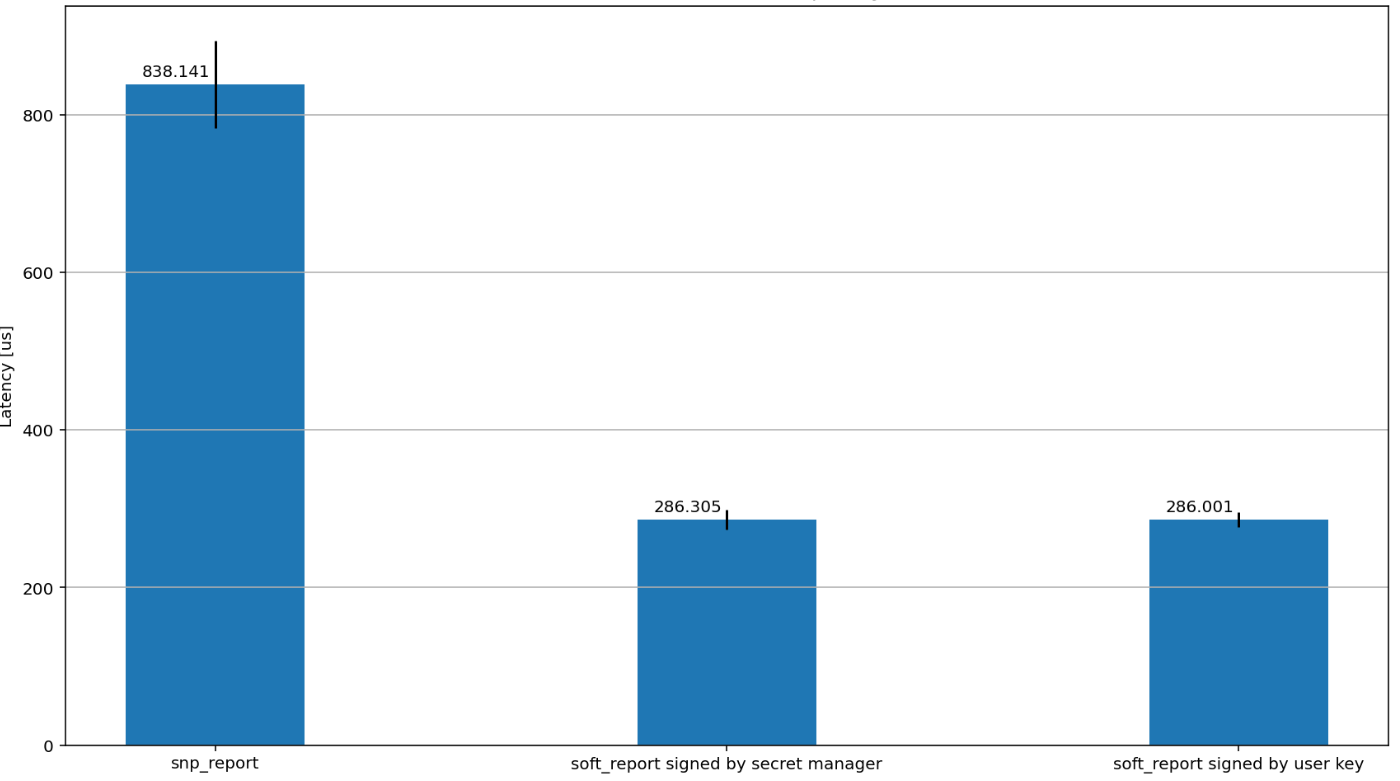
\includegraphics[width=0.5\textwidth]{images/perf_attestation_report_result.PNG}
    \caption[Benchmark result of attestation report syscall]{Qkernel attestation report syscall benchmark Result}
    \label{fig:perf_attestation_report_result}
\end{figure}

Figure~\ref{fig:perf_attestation_report_result} depicts the result. The data reveal that requesting a simulated AMD SEV-SNP report takes approximately 838.141 us, whereas acquiring the two software reports needs only about 286 us. This difference stems from the fact that generating the SEV-SNP report involves expensive operations 
such as virtual machine exit, loading dummy SNP report from the disk, etc. Consequently, obtaining a simulated hardware report is significantly slower than a software report.


\subsection{Micro-benchmark – Qkernel Syscall Interceptor}
\label{bench_Interceptor}

A micro-benchmark is prepared to investigate the latency overhead introduced by intercepting guest system calls~\cite*{benchamark_systemcall_intercetion}. The benchmark executes a system call in a loop using \texttt{SYSCALL} instruction 100,000 times and outputs the average and variance time. The YAML file for deploying this benchmark is 
in repository~\cite*{perf_test_repo}. The benchmark test four system calls: \texttt{getpid}, \texttt{getppid}, \texttt{read}, and \texttt{write}. Since Qkernel already implements process and thread objects, calling getpid or getppid using \texttt{SYSCALL} instruction prompts Qkernel to directly return the corresponding \texttt{pid/ppid} without interference from the 
host. This provides a clear understanding of the overhead introduced by the interceptor. Additionally, the execution time of \texttt{read} and \texttt{write} system calls are measured for confidential and vanilla Quark to evaluate the overhead that the interceptor brought to the host-handled system calls.

\begin{figure}[!htb]
    \centering
    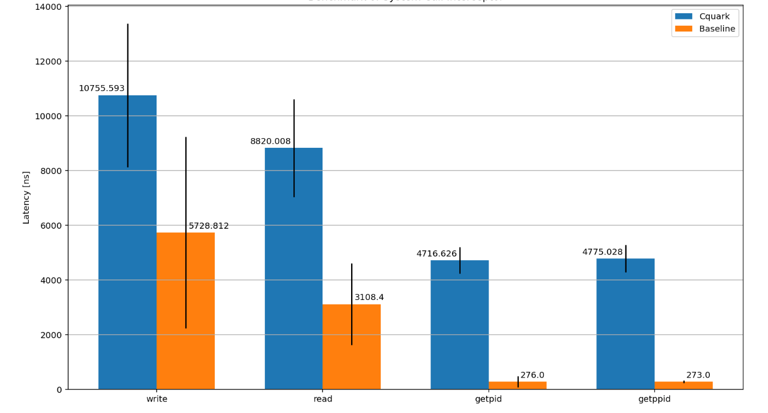
\includegraphics[width=0.5\textwidth]{images/ben_results_syscall_interceptor.PNG}
    \caption[Benchmark result of Syscall Interceptor]{Latency comparison of executing system calls in confidential vs. vanilla Quark. The latency is thereby measured using the guest system call \emph{clock\_gettime(monotonic)}. 
        Each system call is executed 100,000  times in a tight loop. Read and write buffer size is 100 bytes}
    \label{fig:ben_results_syscall_interceptor}
\end{figure}

The test results in Figure~\ref{fig:ben_results_syscall_interceptor} reveal that vanilla Quark takes only around 270 ns to execute a single \texttt{getpid} and \texttt{getppid} call, while confidential Quark takes approximately 4716 ns. This indicates that the guest system call interceptor causes a delay of about 4500 ns per system call. Moreover, a 
comparable latency overhead is introduced for read and write system calls. However, \texttt{read} and \texttt{write} system calls are processed on the host side and take longer. Thus their processing time in confidential Quark rises less significantly than that of \texttt{getpid} and \texttt{getppid}. To summarize, in 
confidential Quark, host-handled system calls (i.e., \texttt{write} and \texttt{read}) and guest-handled-only (e.g.,\texttt{getpid} and \texttt{getppid}) are 1.47x and 17x slower, respectively, compared to vanilla Quark. The overhead of the system call interceptor comes from the access to 
the system call whitelist. Since the whitelist is protected by a lock, each access to the whitelist must acquire this lock first. In addition, the whitelist is kept in an array. Thus, accessing the whitelist has an O(n) time complexity.

\subsection{Micro-benchmark – Speed of Reading File-base Secret}
\label{bench_reading_file_secret}

Compared to vanilla Quark, confidential Quark stores file-type secrets on guest memory. Hence, this benchmark~\cite*{benchamark_filebase_secret} aims to evaluate the performance enhancement achieved from accessing file type secrets in confidential Quark. 
The benchmark measures the total time to perform one \texttt{open} and \texttt{read} operation on a file type secret in confidential and vanilla Quark. The file size is 1302 bytes. The test performs 10,000 open and read operations, and the read buffer size is 100 bytes. The YAML file used to deploy this test 
is in repository~\cite*{perf_test_repo}.

\begin{figure}[!htb]
    \centering
    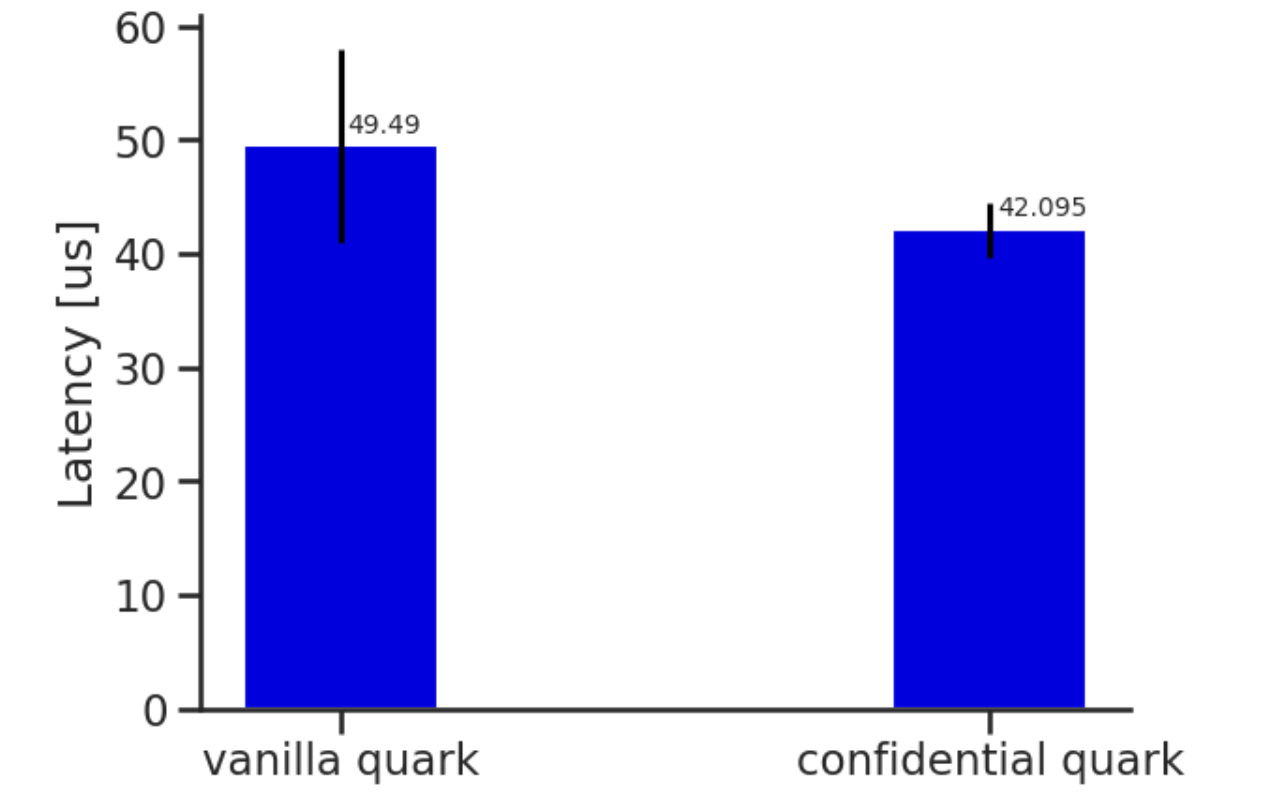
\includegraphics[width=0.5\textwidth]{images/reading_speed_of_file_type_secrets_in_Baseline_and_Cquark.PNG}
    \caption[Speed test for accessing file type secrets in confidential Quark and vanilla Quark]{Speed test for accessing file type secrets in confidential Quark and vanilla Quark.}
    \label{fig:reading_speed_of_file_type_secrets_in_Baseline_and_Cquark}
\end{figure}

The results in Figure~\ref{fig:reading_speed_of_file_type_secrets_in_Baseline_and_Cquark} reveal that confidential Quark's performance in accessing file-type secrets is competitive with vanilla Quark. Surprisingly, the speed in 
confidential Quark is only 1.17 times better. The likely reason for this is that the overhead of the guest system call interceptor in confidential Quark partially offsets the overhead incurred by the VM exit in vanilla Quark.

\subsection{Micro-benchmark – Latency Test for Issuing Instructions to Application}
\label{bench_issuing_Instructions}

This section presents the results of tests conducted to assess the latency of issuing instructions to applications in confidential Quark. The tests involved comparing the latency of sending commands using \emph{kubectl} in confidential and vanilla Quark and the speed comparison test for issuing 
unprivileged and privileged commands in confidential Quark using \emph{kubectl} and \emph{securectl}, respectively. As such, the test framework is extended to issue specific instructions to an application using either \emph{kubectl} or \emph{securectl} while recording command 
execution time~\cite*{benchamark_perf_kubectl}. Besides, each command is issued 1,000 times to ensure dependable results. In the following, four commonly used commands are chosen for the test: \texttt{pwd}, \texttt{ls}, \texttt{cat}, and \texttt{cp}.



\begin{figure}[!htb] 
    \begin{subfigure}[b]{0.5\linewidth}
      \centering
      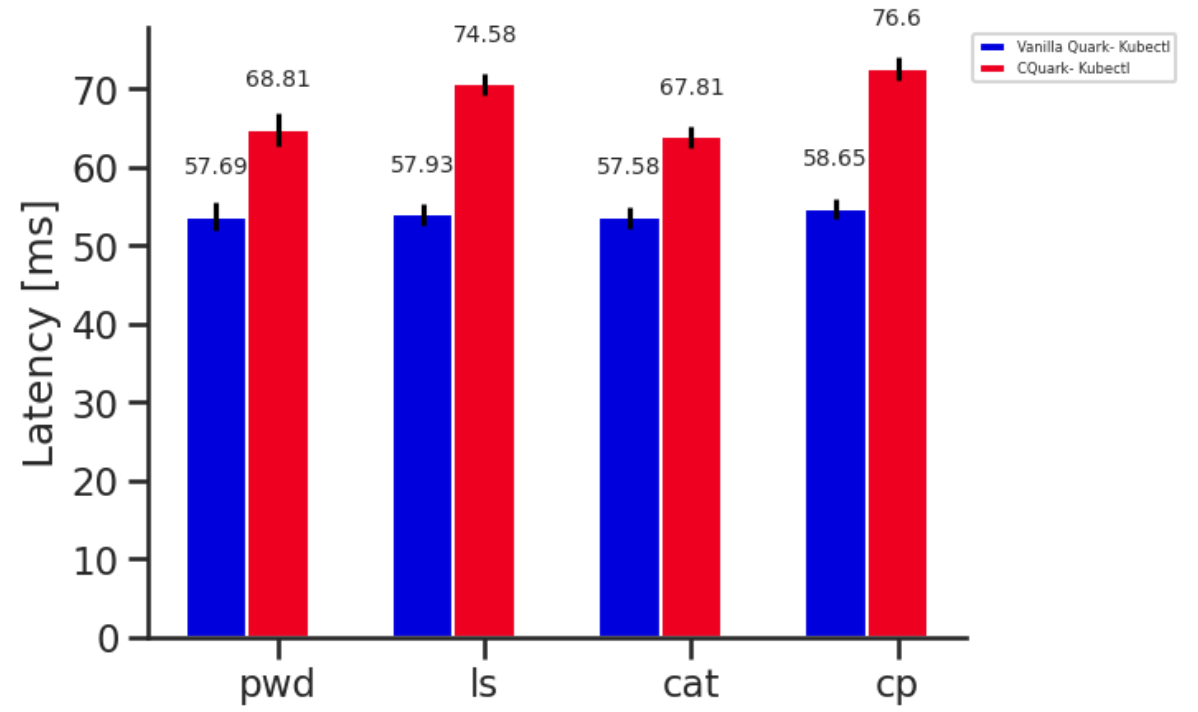
\includegraphics[width=1\textwidth]{images/speed_of_issuing_cmd_in_cquark_upstream_quark.PNG} % first figure itself
      \caption{Issueing commands}
      \label{fig:speed_of_issuing_cmd_in_cquark_upstream_quark}
      \vspace{4ex}
    \end{subfigure}%% 
    \begin{subfigure}[b]{0.5\linewidth}
      \centering
      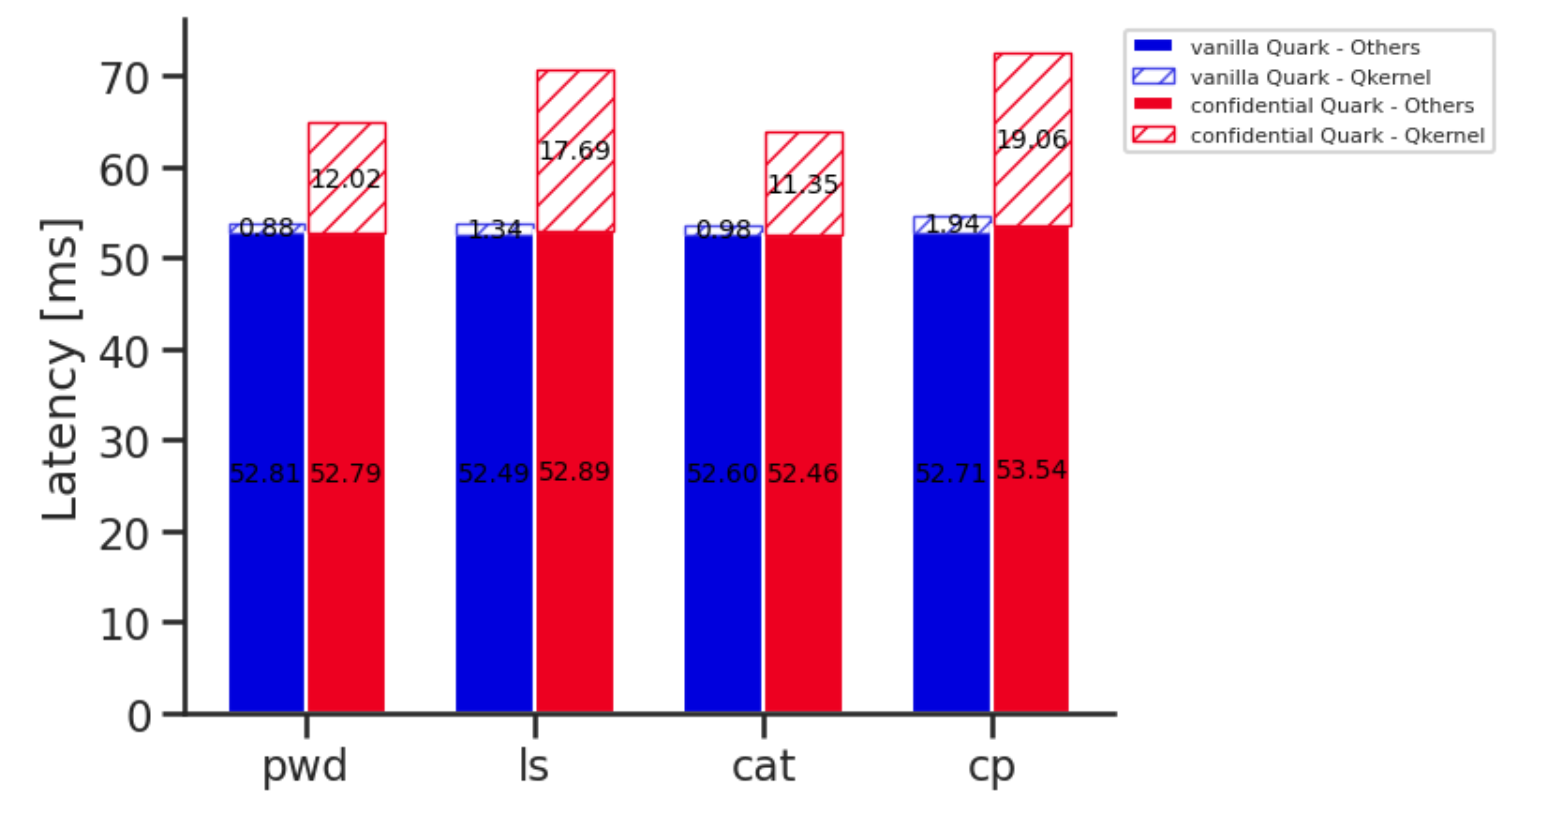
\includegraphics[width=1\textwidth]{images/timeshare_issuing_cmd_in_cquark_upstream_quark_kubectl.png} % second figure itself
        \caption{Time for transferring a command through other components (i.e.,~\emph{kubectl}, Kubernetes, Containerd, and Quark-shim) vs. the time for executing it in Qkernel}
        \label{fig:timeshare_issuing_cmd_in_cquark_upstream_quark_kubectl}
      \vspace{4ex}
    \end{subfigure} 
    \caption{Latency comparison of issuing instruction using kubectl in confidential vs. vanilla Quark}
    \label{fig8} 
\end{figure}


The results in Figure~\ref{fig8} (a) confirm issuing instructions using \emph{kubectl} in confidential Quark is more expensive than in vanilla Quark. Figure~\ref{fig8} (b) exhibits that the additional overhead in confidential Quark comes from the Qkernel 
since it needs to authenticate and access control for each command and measures the command binary. Besides, the guest system interceptor also places an extra burden on Qkernel to execute commands.



\begin{figure}[!htb] 
    \begin{subfigure}[b]{0.5\linewidth}
      \centering
      \centering
      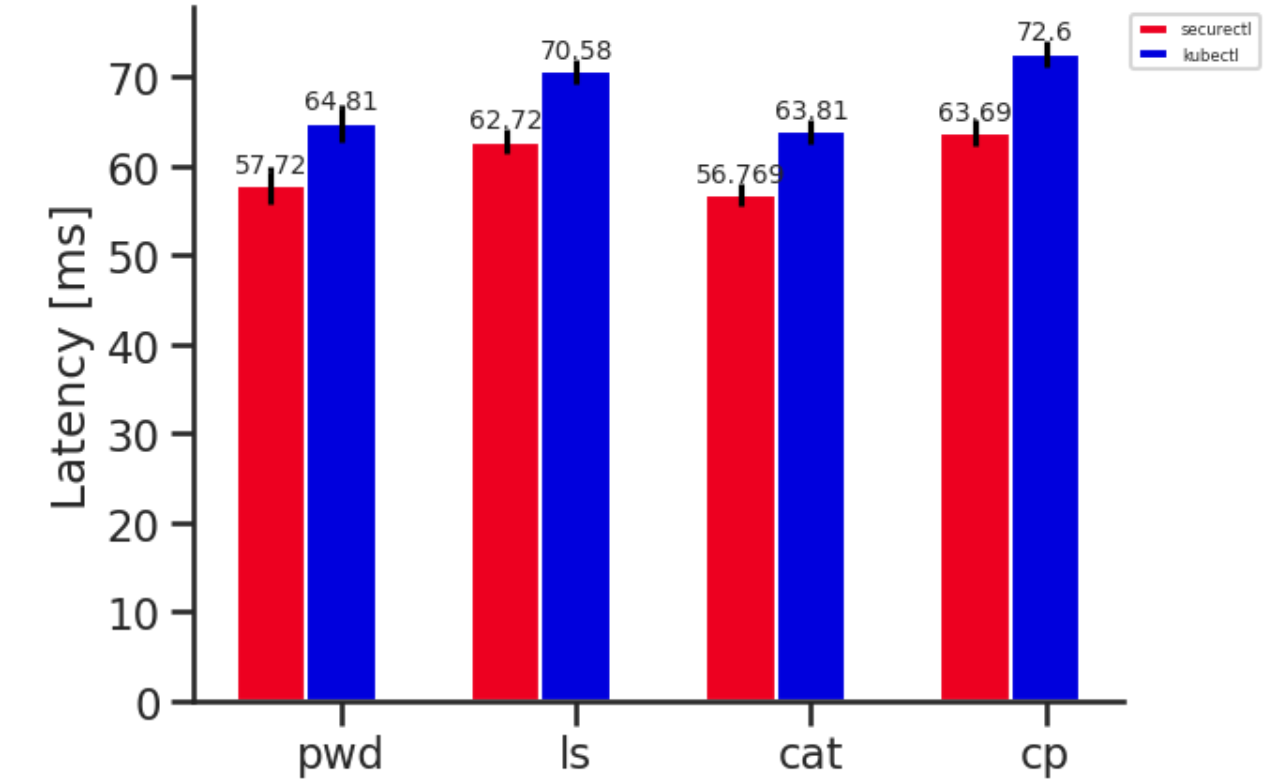
\includegraphics[width=1\textwidth]{images/speed_of_issuing_cmd_in_cquark_kubctl_securectl.png} % first figure itself
      \caption{Issueing commands}
      \label{fig:speed_of_issuing_cmd_in_cquark_kubctl_securectl}
      \vspace{4ex}
    \end{subfigure}%% 
    \begin{subfigure}[b]{0.5\linewidth}
      \centering
      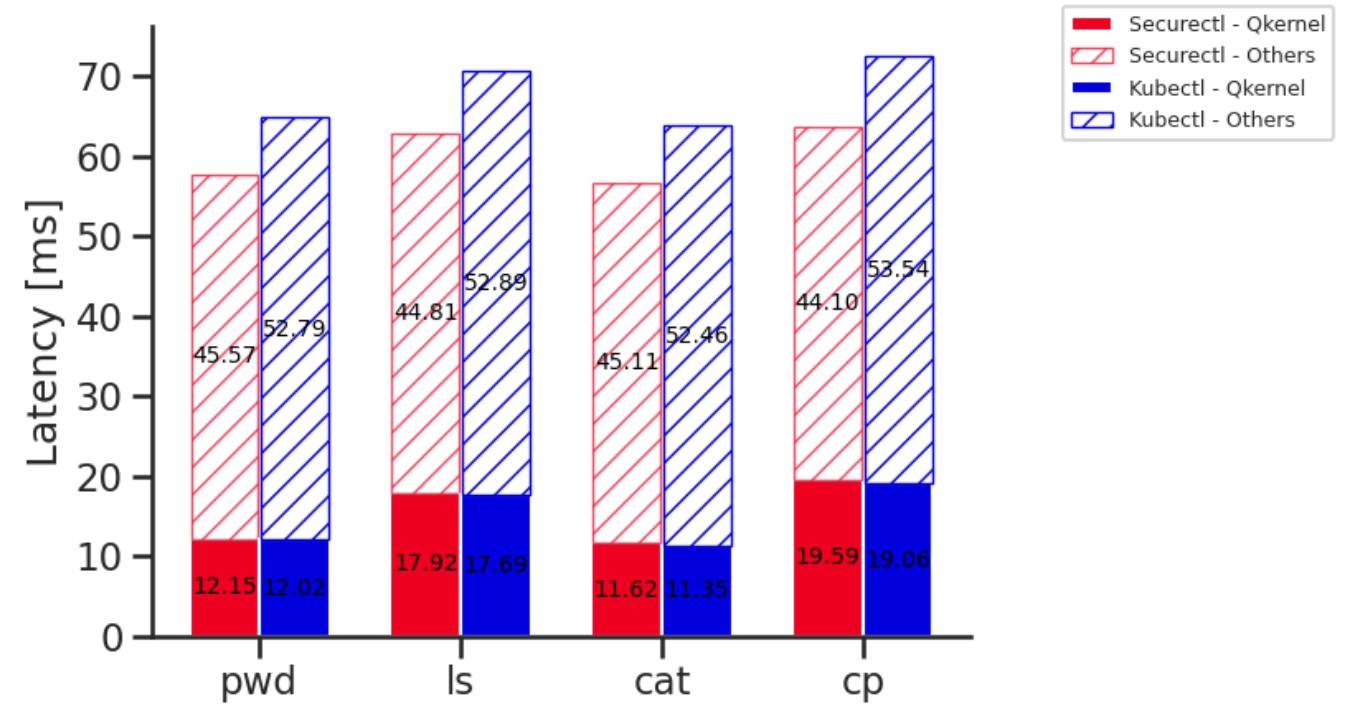
\includegraphics[width=1\textwidth]{images/timeshare_issuing_cmd_in_cquark_kubectl_securectl.png} % second figure itself
      \caption{Time for transferring a command through other components (i.e., ~\emph{kubectl}/~\emph{securectl},  Kubernetes, Containerd, and Quark-shim) vs. the time for executing it in Qkernel}
      \label{fig:timeshare_issuing_cmd_in_cquark_kubectl_securectl}
      \vspace{4ex}
    \end{subfigure} 
    \caption{Latency comparison of issuing privileged vs. unprivileged instructions in confidential Quark}
    \label{fig9} 
\end{figure}



Figure~\ref{fig9} (a) compares the time required to issue privileged and unprivileged commands using~\emph{securectl} and~\emph{kubectl} in confidential Quark. The results show that issuing privileged commands is much faster than issuing unprivileged commands. 
This finding is counterintuitive since privileged instructions require additional cryptographic protection, which implies executing additional code. To investigate this further, the time for transferring a command through other components (i.e.,~\emph{kubectl}/\emph{securectl},  Kubernetes, Containerd, and Quark-shim) and the time for executing it in Qkernel 
are measured.  The results in Figure~\ref{fig9} (b) show that Qkernel takes roughly one millisecond longer to execute privileged commands than it does to execute unprivileged commands. However, non-privileged level commands spend significantly more 
time in the other components than privileged commands (dashed-filled boxes). The only difference between the other components for the privileged and unprivileged commands is the tool used to issue the instructions (i.e., ~\emph{kubectl}/\emph{securectl}). This means that \emph{securectl} is more 
lightweight than \emph{kubectl} and thus offsets the cryptographic protection overhead of privileged commands.






\subsection{Micro-benchmark – Latency Test for Accessing Binary-mapped Memory Region}
\label{accesiing_binary_mapped_memory}

Instead of lazy loading a process's executable and shared libraries while the process is running, confidential Quark preloads these files into the guest. This avoids page error handling for loading these files at program runtime. As such, this subsection compares the speed of access to binary-mapped memory regions at runtime 
in the confidential and vanilla Quark. The benchmark utilizes a program~\cite*{benchamark_micro} containing~\emph{a global initialized array} and a~\emph{for} loop. The program can access the array within the~\emph{for} loop using four access modes: \texttt{random read}, \texttt{random write}, 
\texttt{sequential read}, and \texttt{sequential write}.  The test is conducted in three binary data segment mapped memory sizes, i.e., 5MB, 10MB, and 100MB. For each case, the benchmark framework~\cite*{benchamark_framework} executes the program 30 times and calculates the average cost of accessing the array. Note that the size of the binary data segment 
mapped memory region is controlled by the size of the array. 


\begin{figure}[!htb] 
    \begin{subfigure}[b]{0.5\linewidth}
      \centering
      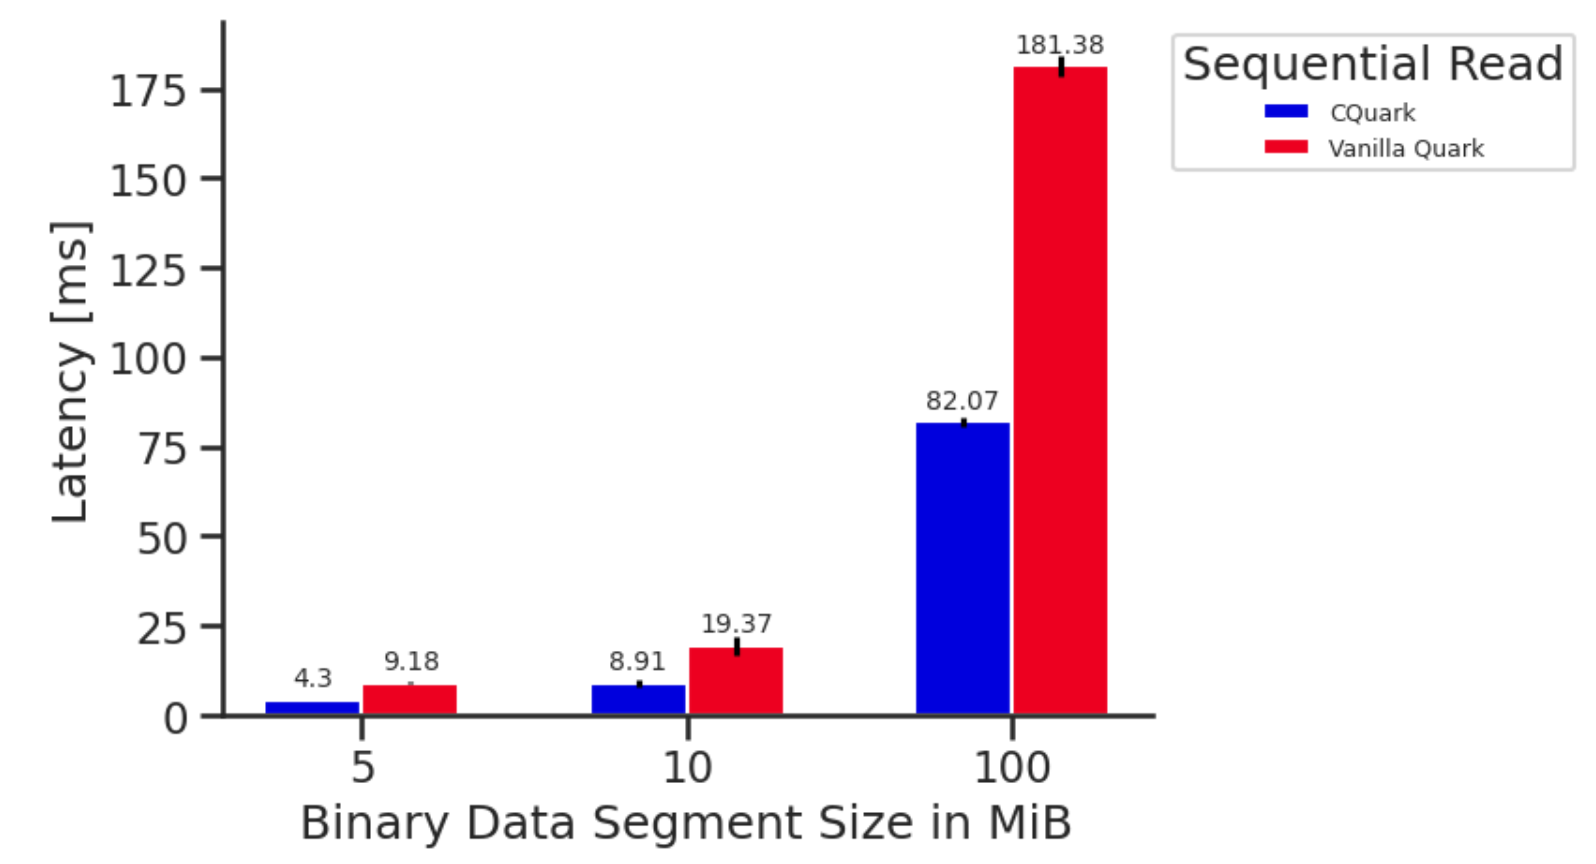
\includegraphics[width=0.9\linewidth]{images/Sequential_Read.PNG} 
      \caption{Sequential Read} 
      \label{fig7:a} 
      \vspace{4ex}
    \end{subfigure}%% 
    \begin{subfigure}[b]{0.5\linewidth}
      \centering
      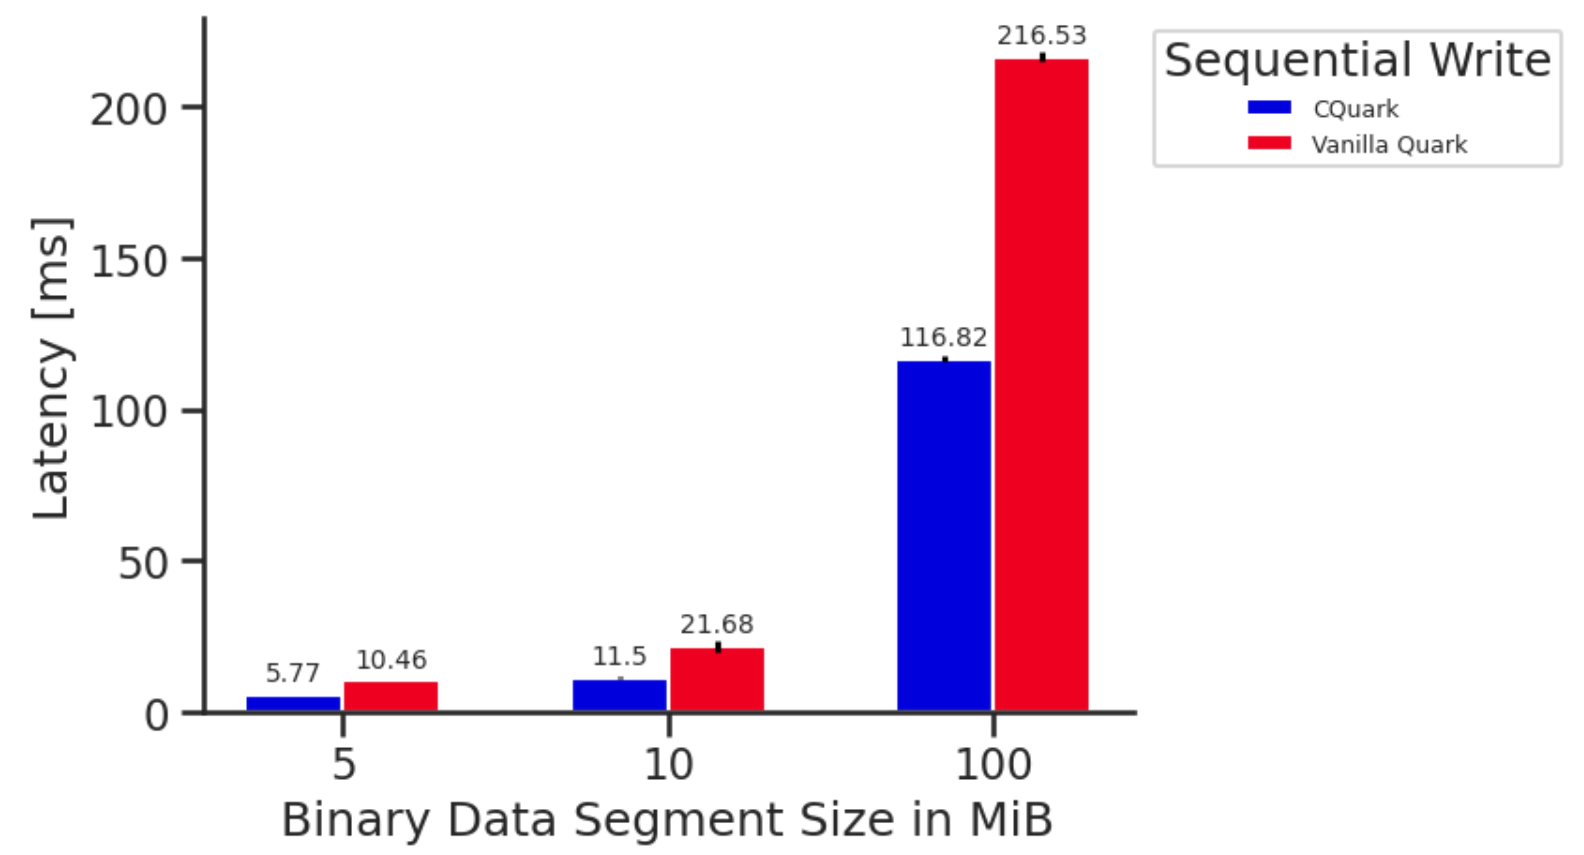
\includegraphics[width=0.9\linewidth]{images/Sequential_Write.PNG} 
      \caption{Sequential Write} 
      \label{fig7:b} 
      \vspace{4ex}
    \end{subfigure} 
    \begin{subfigure}[b]{0.5\linewidth}
      \centering
      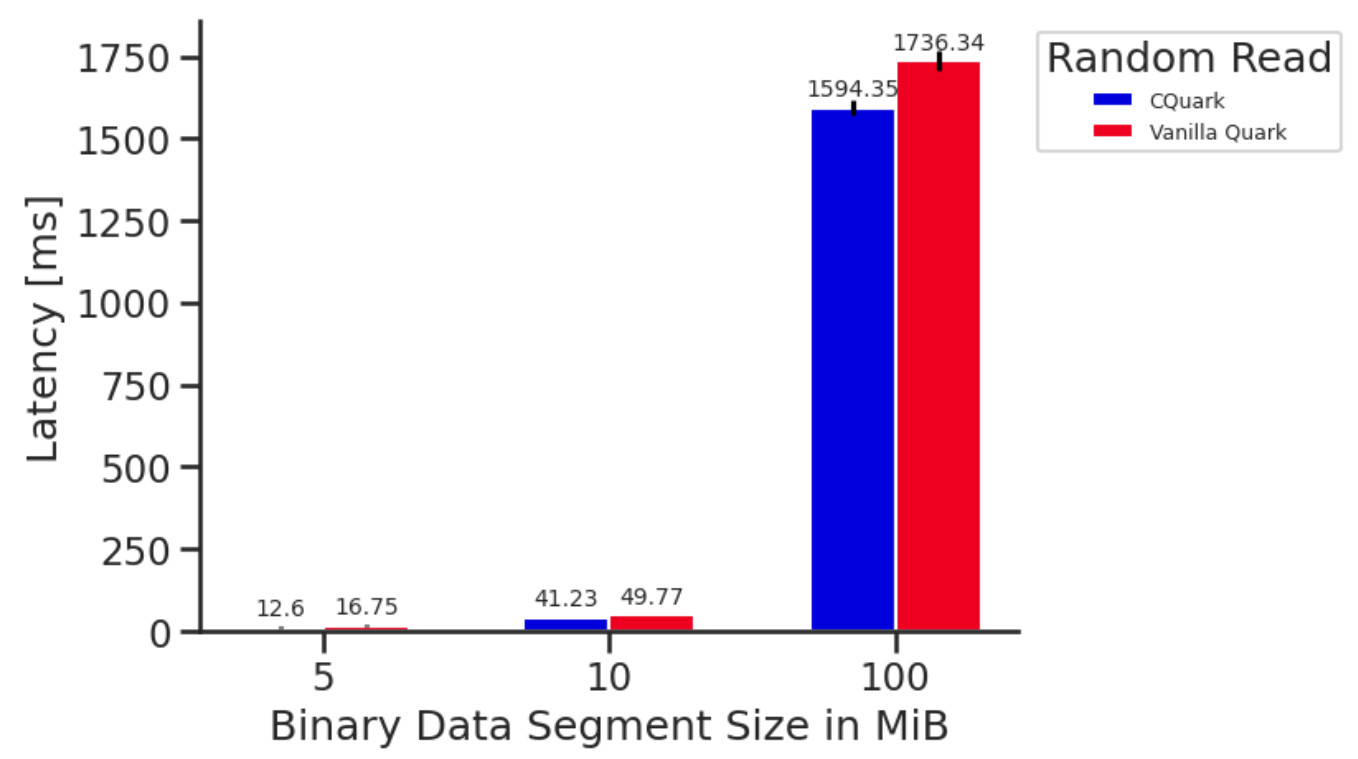
\includegraphics[width=0.9\linewidth]{images/Random_Read.PNG} 
      \caption{Random Read} 
      \label{fig7:c} 
    \end{subfigure}%%
    \begin{subfigure}[b]{0.5\linewidth}
      \centering
      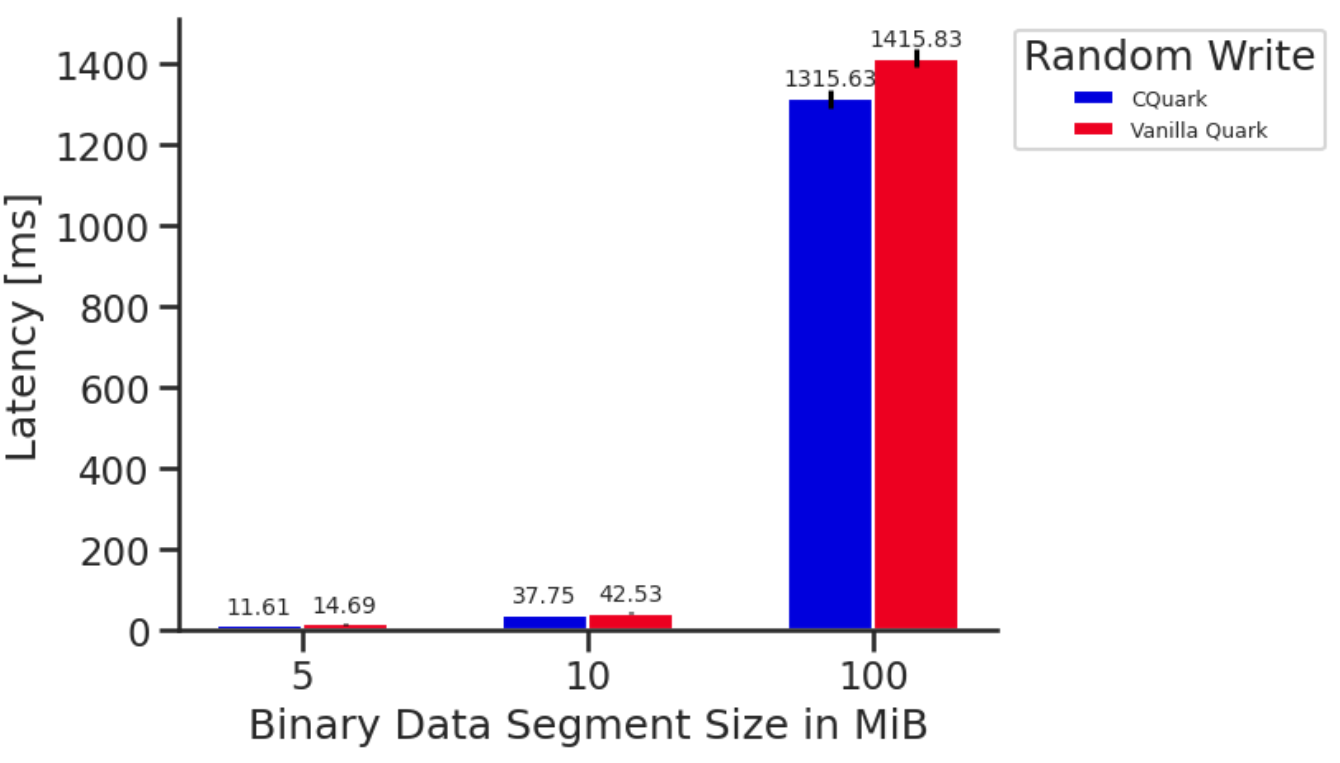
\includegraphics[width=0.9\linewidth]{images/Random_Write.PNG} 
      \caption{Random Write} 
      \label{fig7:d} 
    \end{subfigure} 
    \caption{Benchmark Result - Latency Test for accessing binary-mapped memory region}
    \label{fig7} 
\end{figure}



The results shown in Figures~\ref{fig7} (a) and~\ref{fig7} (b) indicate that the sequential access in the confidential Quark is more than 1.8 times faster than in the vanilla Quark. The reason is that confidential Quark preloads the binary into the guest memory before the program launches, thus avoiding page 
fault handling at runtime. For the same reason, random reads and writes in confidential Quark are about 1.08 times faster than in vanilla Quark (Figure ~\ref{fig7} (c) and Figure ~\ref{fig7} (d)).


\subsection{Micro-benchmark – Latency Test for Application Startup}
\label{micro_app_start_up}

This subsection evaluates the latency overhead that the shield imposes on application startup. As described in Chapter~\ref{sec:implementation}, two factors may affect the application startup time: the number of file type secrets and the data size measured by the software measurement manager. Therefore, 
the following three tests are performed in this subsection. First, a baseline is established by setting the number of file type secrets to zero and running the hello world program in Listing~\ref{code2} with an array length equal to 1024 * 1024. 
In experiment 2, the number of file type secrets is increased to observe the change in program startup time. Experiment 3 examines the effect of increasing the binary size on program startup time.


    
The test framework~\cite*{benchamark_framework} is extended to start and terminate the application iteratively. It measures the mean and variance of the program startup time and evaluates the overhead imposed by the components in the shield. These components include the remote attestation and 
provisioning agent,  secret injector,  hardware evidence driver, and software measurement manager. Additionally, the statically linked program from Listing~\ref{code2} is utilized as the test workload. It contains a global initialized array to regulate the binary data segment size. 
The framework will run the application 100 times. For the methodology for measuring the overhead introduced by the shield component, please refer to  subsection~\ref{Hardware_and_Software_Setup}.

\begin{lstlisting}[language=C,frame=single,caption=Hello World Program Variant,label=code2]
  #define ARRAY_LEN (unsigned long)(1024*1024*100)    
  char array[ARRAY_LEN] = {[ 0 ... (1) ] = 'a'} ;
  int main() {     
      printf("Hello, World!\n");
      return 0;
  }
  \end{lstlisting}
  

\begin{figure}[!htb]
    \centering
    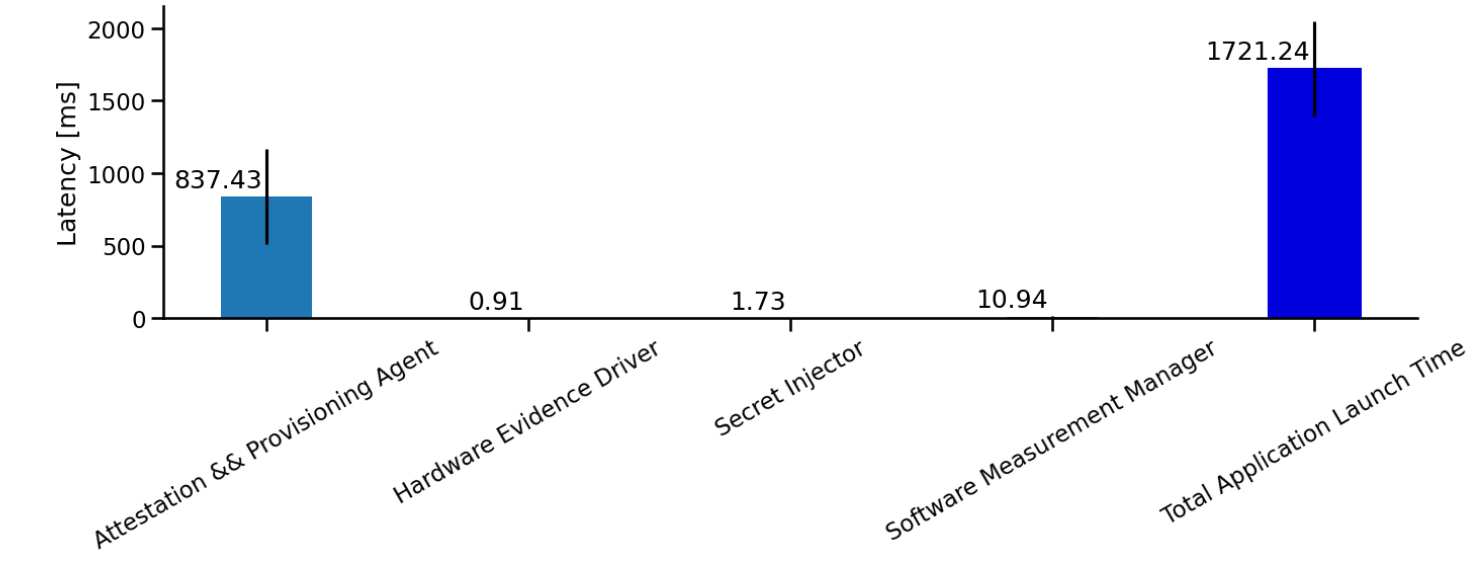
\includegraphics[width=0.7\textwidth]{images/application_start_microtest_baseline_time_overhead_each_cmp.PNG}
    \caption[Baseline: latency overhead introduced by shielding layer]{Baseline: latency overhead introduced by shielding layer}
    \label{fig:application_start_microtest_baseline_time_overhead_each_cmp}
\end{figure}


\begin{table}[!htb]
    \centering
    \footnotesize
    \caption{Software measurement manager measured data during application startup\strut}
    \begin{tabularx}{1\textwidth}{@{} l L L L L L L@{}}
    \toprule
        Matrics    & ELF &  Shared Lib   & Qkernel Config File    & Public Key of Secret Manager  & Total\\
    \midrule

        \vn{Measurement}     &  1.447 MiB    &   0 MiB  &   534 Byte      &2017 Byte  & 1.449 MiB\\
    \bottomrule
    \end{tabularx}
    \label{table: Measurement_For_Hello_world}
\end{table}


The baseline results in Figure~\ref{fig:application_start_microtest_baseline_time_overhead_each_cmp} illustrate that approximately 50\% of the program's startup time is allocated for initializing the shield's components. Notably, the remote attestation and provisioning agent contributed the most to 
the latency overhead, which is expected since it must establish a TLS connection with the relying party, complete the remote attestation process, and retrieve the secrets. The secret injector, hardware evidence driver, introduces a latency overhead of 0.90 ms and 1.73 ms. However, this latency is 
negligible compared to the overhead caused by the attestation agent (837 ms). In addition, the data in Table~\ref{table: Measurement_For_Hello_world} indicates that the software measurement manager measured approximately 1.449 MiB of data during program startup, resulting in an overhead of only 
10 milliseconds. 

\begin{figure}[!htb]
    \centering
    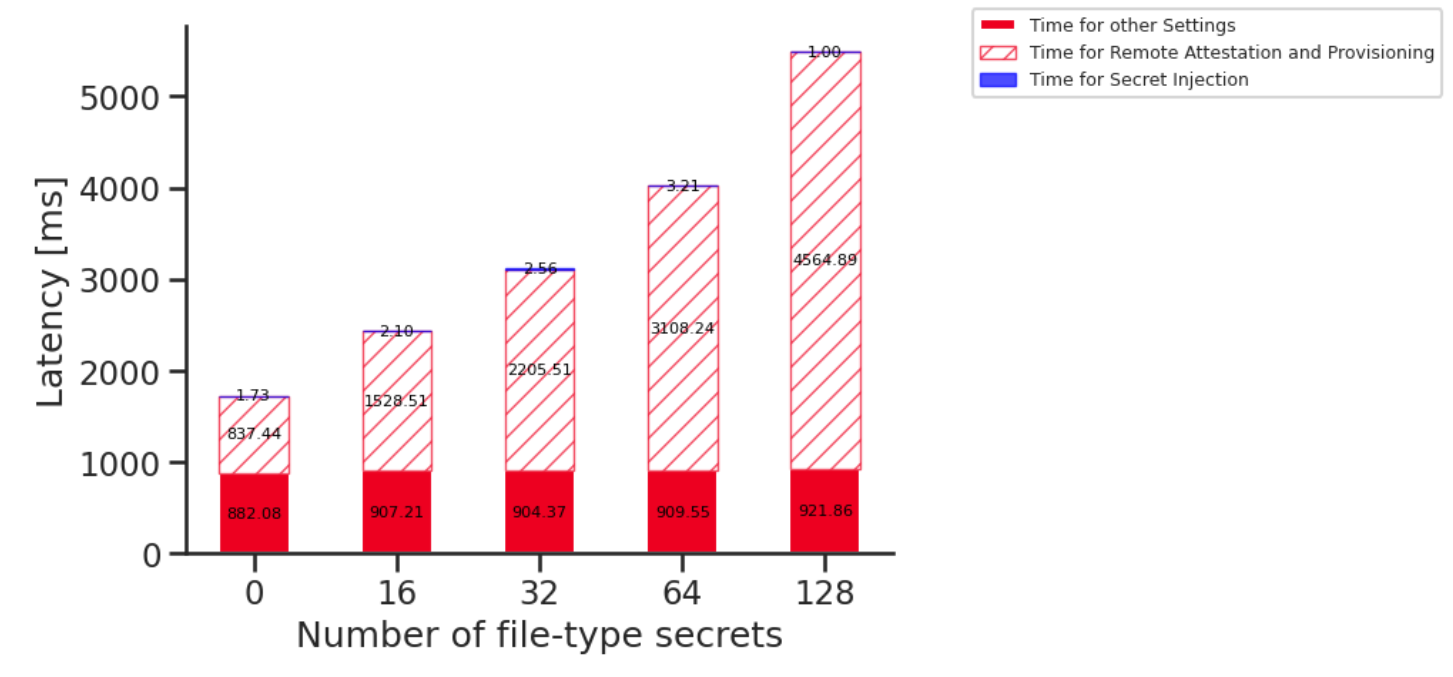
\includegraphics[width=0.8\textwidth]{images/startup_time_change_as_file_type_secret_increasing.PNG}
    \caption[Distribution of the time consumed by attestation \&\& provisioning agent, secret injector and others in the application startup]{Distribution of the time consumed by attestation \&\& provisioning agent, secret injector and others in the application startup}
    \label{fig:startup_time_change_as_file_type_secret_increasing}
\end{figure}

Figure~\ref{fig:startup_time_change_as_file_type_secret_increasing} shows that the latency overhead from the remote attestation and provisioning agent is proportional to the number of file type secrets. 
This is because the agent must perform one HTTP + TLS operation for each file. When the number of file-type secrets reaches 128, the overhead associated with the agent becomes astounding, reaching 4500 ms, accounting for over 70\% of the total program startup time.
\begin{figure}[!htb]
    \centering
    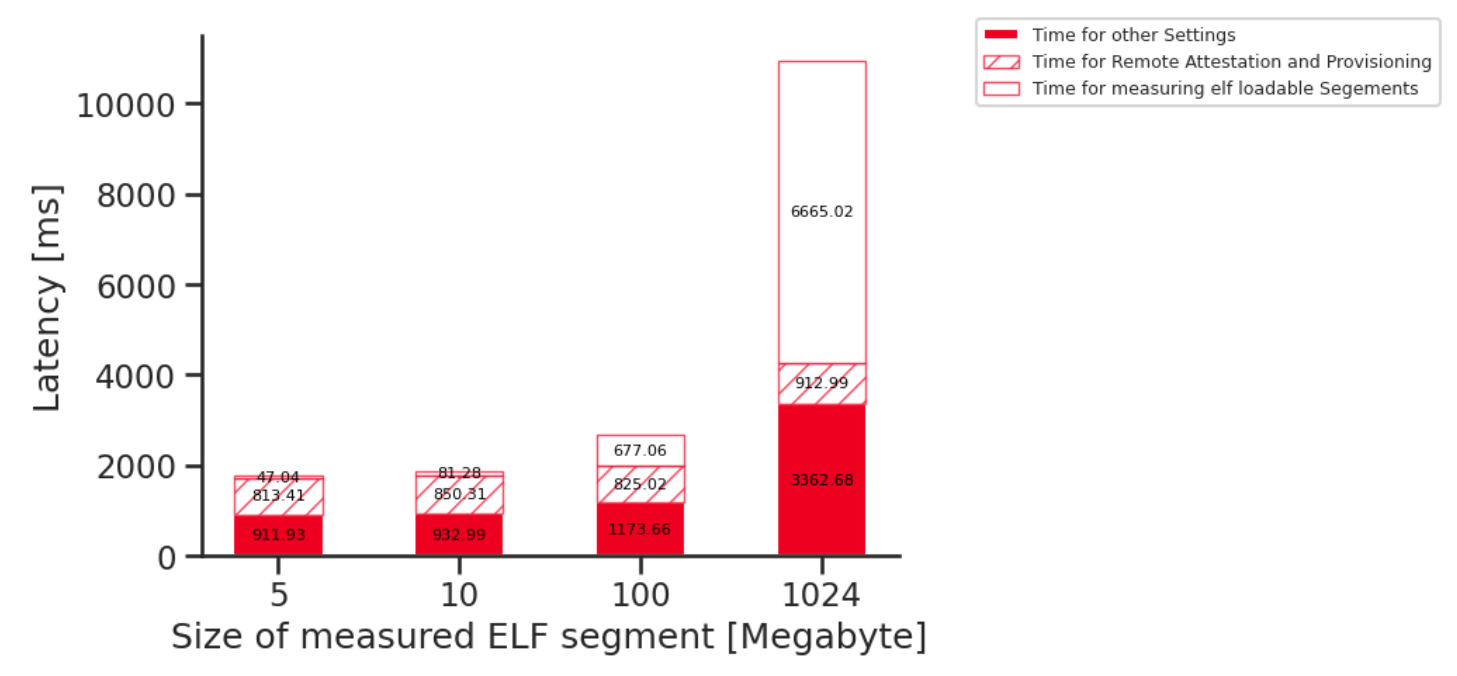
\includegraphics[width=0.8\textwidth]{images/startup_time_change_as_elf_size_increasing.PNG}
    \caption[Distribution of the time consumed by software measurement manager and others in the Application Startup]{Distribution of the time consumed by software measurement manager and others in the application startup}
    \label{fig:startup_time_change_as_elf_size_increasing}
\end{figure}


Figure~\ref{fig:startup_time_change_as_elf_size_increasing} shows that the latency overhead of the software measurement manager is proportional to the size of the binary. Besides, when the measured data is less than or equal to 100 MiB, the latency overhead of the software measurer is lower than the 
overhead introduced by the remote attestation and provisioning agent.


\subsection{Macro-Benchmark– Application Life Cycle Performance Benchmark}
\label{macri_app_start_up}

This subsection evaluates the performance of running real-world applications in confidential and vanilla Quark. The Nginx~\cite*{nginx} and Redis~\cite*{redis} are chosen as test subjects and their startup time, exit time, and runtime throughput are measured. At program runtime, the Apache HTTP 
Server Benchmarking Tool~\cite*{ab} and Redis-benchmark~\cite*{Redis_benchmark} are used to generate workloads for Nginx and Redis, respectively.

Regarding the benchmarking methodology, the testing framework~\cite*{benchamark_framework} is extended to repeatedly launch the target application 100 times, record its startup and exit times, and the results of Redis and Apache benchmarks. Redis and Apache benchmarks are set to issue 1,000,000 
requests using 50 concurrent clients to Redis and Nginx, respectively. In addition, the file size requested by Apache benchmark from Nginx is 181 bytes. Both applications fetch the shield policy from the secret manager only.


 \begin{figure}[!htb]
  \centering
  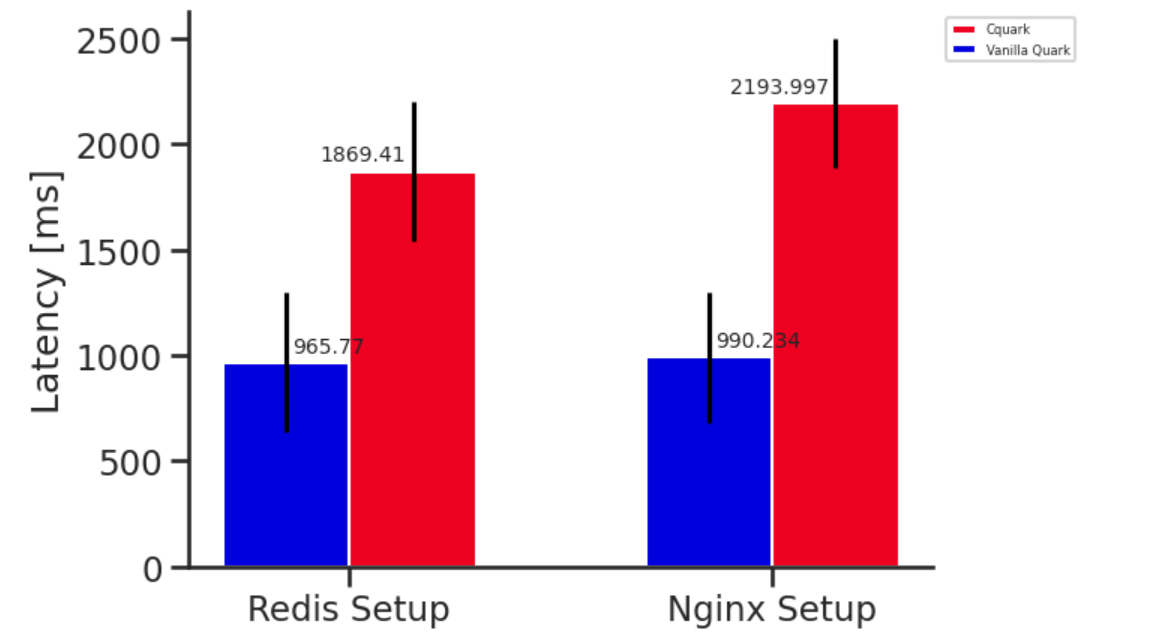
\includegraphics[width=0.5\textwidth]{images/reds_nginx_startup_comp.PNG}
  \caption[Redis \&\& Nginx startup time in confidential vs vanilla Quark]{Redis \&\& Nginx startup time in confidential vs vanilla Quark}
  \label{fig:reds_nginx_startup_comp}
\end{figure}


\begin{figure}[!htb]
  \centering
  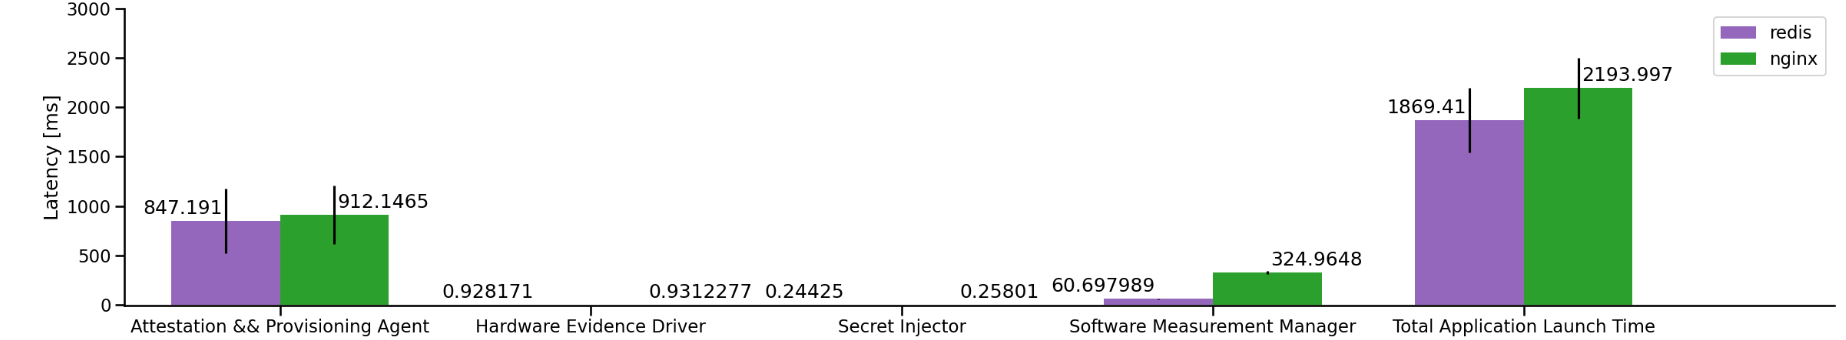
\includegraphics[width=0.8\textwidth]{images/time_disribution_startup_redis_nginx.PNG}
  \caption[Redis \&\& Nginx startup time in confidential vs vanilla Quark]{Redis \&\& Nginx startup time in confidential vs vanilla Quark}
  \label{fig:time_disribution_startup_redis_nginx}
\end{figure}



\begin{table}[!htb]
  \centering
  \scriptsize

  \begin{tabularx}{1\textwidth}{@{} l L L L L L L@{}}
  \toprule
      Matrics    & ELF &  Shared Library   &Qkernel Config File    & Public Key of Secret Manager  & Total Measurement\\
  \midrule

      \vn{Measurement for Redis}     &  3.64 MiB   &   12.61 MiB  &   534 Byte      &2017 Byte   & 16.25 MiB\\
      \vn{Measurement for Nginx}     &  5.5 MiB    &   61.64 MiB  &   534 Byte      &2017 Byte   & 67.14 MiB\\
  \bottomrule
  \end{tabularx}
  \caption{Software measurement manager measured data during application startup}
  \label{table:Measurement_For_Nginx_Redis}
\end{table}

The results in Figure~\ref{fig:reds_nginx_startup_comp} indicate that confidential Quark takes about twice as long as vanilla Quark to complete the application setup. This result is reasonable because the confidential Quark must perform additional operations such as remote attestation and 
measuring data loaded from the host. When comparing the startup times of Nginx and Redis in confidential Quark, it is evident that Nginx takes about 324 ms longer than Redis. Fig~\ref{fig:time_disribution_startup_redis_nginx} shows that the difference mainly comes from the latency overhead 
difference of the software measurement manager and the remote attestation and provisioning agent, i.e., 424 ms and 65 ms, respectively. Since both applications retrieve the same number of secrets from the secret manager, the difference in remote attestation and provisioning 
agent's overhead should come from the network jitter. In addition, Table~\ref{table:Measurement_For_Nginx_Redis} shows that the software measurement manager measured 67.14 and 16.25 Mib in Nginx and Redis, respectively. Because the software measurement manager has to measure more data in 
Nginx, its latency overhead is larger in Nginx. 

\begin{figure}[!htb]
  \centering
  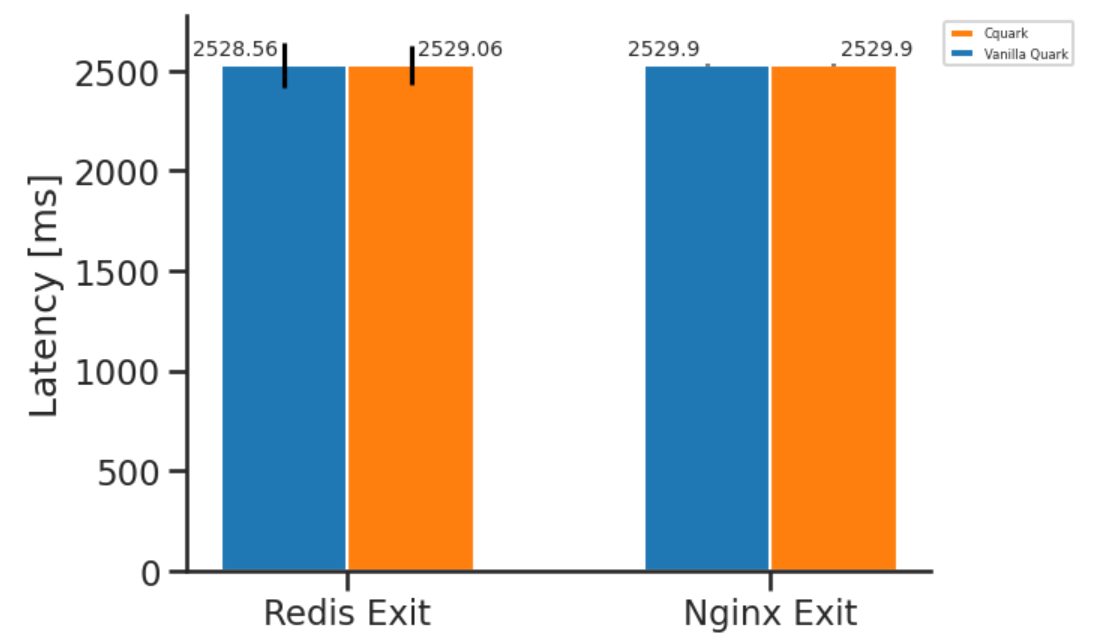
\includegraphics[width=0.5\textwidth]{images/reds_nginx_exit_comp.PNG}
  \caption[Redis \&\& Nginx Exit Time in Cquark vs vanilla Quark]{Redis \&\& Nginx Exit Time in Cquark vs vanilla Quark}
  \label{fig:reds_nginx_exit_comp}
\end{figure}
Figure~\ref{fig:reds_nginx_exit_comp} shows that the exit time for Redis and Nginx is around 2529 milliseconds in both confidential and vanilla Quark, as confidential Quark does not modify the critical path for program exit.
\begin{figure}[!htb]
  \centering
  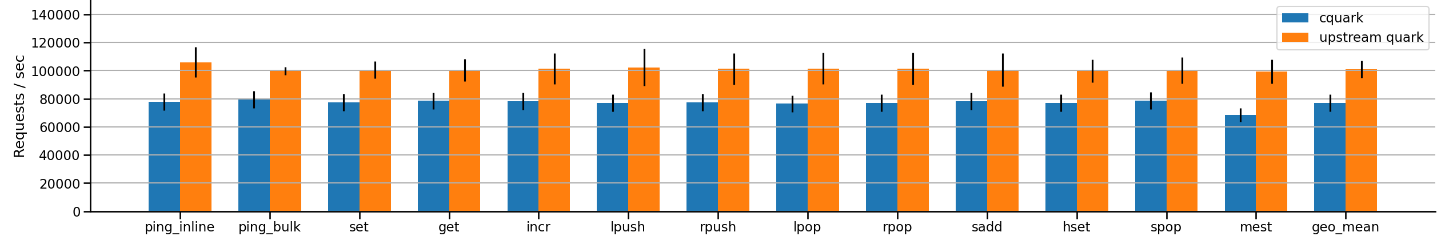
\includegraphics[width=1\textwidth]{images/redis_throughput.PNG}
  \caption[Redis Throughout Test]{Redis Throughout Test Result}
  \label{fig:redis_throughput}
\end{figure}


\begin{figure}[!htb]
  \centering
  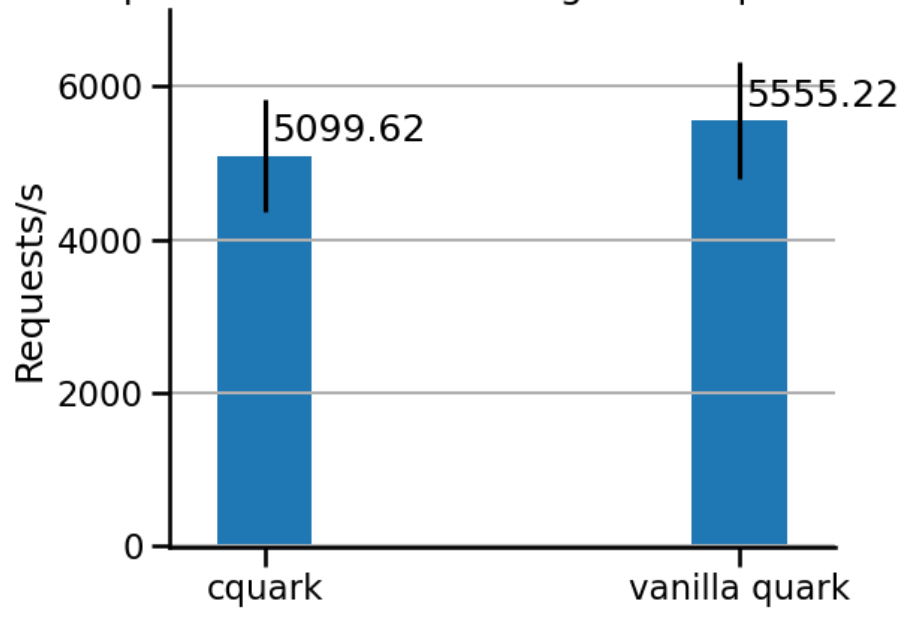
\includegraphics[width=0.5\textwidth]{images/nginx_throughput.PNG}
  \caption[Nginx Throughout Test]{Nginx Throughout Test Result}
  \label{fig:nginx_throughput}
\end{figure}

The throughput test results for Redis and Nginx are shown in Figure~\ref{fig:redis_throughput} and Figure~\ref{fig:nginx_throughput}. It shows that executing Redis and Nginx in confidential Quark leads to about 22\% and 10\% performance degradation, respectively. 
The possible reason for this impact is the overhead introduced by intercepting guest system calls.


\subsection{Trust Computing Base}\label{tcb}

This subsection evaluates the \acrshort{TCB} overhead introduced by the shield and compares the \acrshort{TCB}  sizes of confidential Quark and Kata containers~\cite*{Kata-Containers}. To this end, the lines of code and the size of the guest kernel binary for confidential and 
vanilla Quark are compared. Note that the guest kernel binary comprises the code from 3 components, Qkernel, Qlib, and the shielding layer. In comparing the \acrshort{TCB} sizes of confidential Quark and Kata containers, the binary sizes of the guest assets is utilized as a reference. The assets for 
confidential Quark are the guest kennel (Qkernel) binary, while the assets for the Kata containers include the Kata agent~\cite*{kata_agent}, OVMF~\cite*{ovmf}, and the Linux kernel. Besides, the strip utility~\cite*{strip} is utilized to remove unused symbols from the binaries to ensure fairness.

\begin{table}[htbp]
  \centering
\begin{tabular}{lrrrcrrr}\toprule
  \hline
  \multicolumn{3}{c}{Vanilla Quark}&&\multicolumn{3}{c}{Confidential Quark}\\
  \cline{1-3}\cline{5-7}
  $Component$ & $LoC$ & $Size$$^{3}$ && $Component$ & $LoC$ & $Size$$^{3}$\\
\midrule
   Qkernel &32487 & -&& Qkernel&32487&-\\
   Qlib &85128  & -&&Qlib&  86609 &-\\
   Shield  & 0 & - && Shield&2805&-\\

   \midrule
    Total  & 117615& 3.1MiB&& & 121901 &  4.6 MiB\\
    \bottomrule
\end{tabular}

\caption{Comparison of the LoC and the guest kernel binary size of vanilla and confidential Quark}
\label{table:tcb_size_quark_vs_cquark}
\end{table}


Table~\ref{table:tcb_size_quark_vs_cquark} summarizes the \acrshort{TCB} size in confidential and vanilla Quark. Vanilla Quark's guest kernel has 117615 lines of code and generates a statically linked binary of 3.10 MB. In confidential Quark, the shield adds 4286 lines of code to the guest kernel, 
bringing the total number of lines of code to 121901, and the binary reaches 4.6 MB. Overall, the shield increases the size of the guest binary by a factor of 1.48 compared to vanilla Quark. 
The reason for this is that the guest binary is statically linked, and the shield adds a lot of libraries to the guest binary.  

\begin{table}[htbp]
  \centering
\begin{tabular}{lrrcrr}\toprule
  \hline
  \multicolumn{2}{c}{Kata Container}&&\multicolumn{2}{c}{Confidential Quark}\\
  \cline{1-2}\cline{4-5}
  $Component$  & $Size$$^{3}$ && $Component$  & $Size$$^{3}$\\
\midrule
   Guest Kernel &47.16 MiB && Guest kernel &4.6 MiB\\
   OVMF   & 4 MiB && &   &\\
   Kata agent  & 22.65MiB  && &&\\

   \midrule
      & 73.81 MB&& &   4.6 MiB\\
    \bottomrule
\end{tabular}

\caption{TCB size comparison between kata container vs. confidential quark in terms of binary size of guest assets \strut}
\label{table:tcb_size_quark_vs_kata}
\end{table}

Table~\ref{table:tcb_size_quark_vs_kata} compares the size of \acrshort{TCB}s in the Kata containers and the confidential Quark. In the Kata containers, the binary sizes of the Kata agent, OVMF, and guest kernel are 22.65 MB, 4.0 MB, and 47.16 MB, respectively. The total \acrshort{TCB} size is 
73.81 MB, about 16 times that of the confidential Quark.

\subsection{Summary of Quantitative Analysis}
\label{sec:qualitativ_sum}
This section evaluated the latency and throughput overhead introduced by the shield using different benchmarks.

Subsection~\ref{Attestation_Report_Syscall} found that obtaining the simulation hardware report is much slower than getting the other two software reports. Subsequently, the benchmark result in subsection~\ref*{bench_Interceptor} showed that the guest system interceptor 
imposes an overhead of 1.47x and 17x for host-handled and guest-handled system calls, respectively. Furthermore, Subsection~\ref{bench_reading_file_secret} revealed that in the confidential Quark, the speed of accessing file-type secrets is 1.17 times higher than in the vanilla Quark.
Subsection~\ref{bench_issuing_Instructions} then demonstrated that issuing commands using \emph{kubectl} in confidential Quark is about 20\% slower than in vanilla Quark. On the other hand, using \emph{securectl} to issue commands is 1.1 times faster than using \emph{kubectl} in confidential 
Quark since \emph{securectl} is more lightweight than \emph{kubectl}.

Then after estimating the performance of accessing binary-mapped memory regions, Subsection~\ref{accesiing_binary_mapped_memory} observed that confidential Quark outperforms vanilla Quark in this regard. Sequential access in confidential Quark is more than 1.86 times faster, while random reading and 
writing of binary-mapped memory regions exhibit approximately 1.08 times faster speed in confidential Quark. Regarding the application startup time, Subsection~\ref*{micro_app_start_up}’s evaluation results indicated that the attestation and provisioning agent constitutes the bulk of the overhead when the size of the measurement data is less than 100 MB. 
Furthermore, when the number of file type secrets reaches 128, the overhead associated with the remote attestation and provisioning agent reaches 4500 ms, more than 70\% of the total program startup time.

Subsection~\ref*{macri_app_start_up} performed macro-benchmarks using Nginx~\cite*{nginx} and Redis~\cite*{redis}. The findings demonstrated that Redis and Nginx require 1.93X and 2,21X startup times in confidential Quark than in vanilla Quark, respectively. 
In terms of application exit time, Redis and Nginx exhibit almost the same performance when running in confidential and vanilla Quark. Regarding the throughput, the test results indicated that Nginx and Redis running in confidential Quark encounter performance declines of approximately 10\% and 20\%, 
respectively.

About TCB overhead, Subsection~\ref{tcb} showed that the shield increase the binary of the Quark guest kernel by about 1.47 times. Nevertheless, the TCB of confidential Quark is roughly one-sixteenth of the size of the Kata containers. 

\section{Summary}
This chapter conducted qualitative and quantitative analyses to evaluate the confidential Quark~\ref{sec:implementation}. The qualitative analysis explained how confidential Quark mitigates the vulnerabilities of the OCI runtime interface listed in Section~\ref*{sec:security_analyse_oci_summary}. 
Regarding the quantitative analysis, a testing framework~\cite*{benchamark_framework} was developed to characterize the performance of confidential Quark. The results showed that confidential Quark incurs significant latency overhead compared to vanilla Quark. 
This overhead is visible in longer program creation times, reduced runtime program throughput, reduced speed of issuing instructions to the program, increased \acrshort{TCB} size, etc. 
Note that the summary of qualitative and quantitative analyses can be found in Section~\ref*{sec:eva_qualitativ_summary} and ~\ref{sec:qualitativ_sum}, respectively. 
\cleardoublepage

